\documentclass[]{article}
\usepackage{geometry}
\geometry{a4paper, margin=1in}
\usepackage{amssymb}
\usepackage{multirow}                                                      % you want to use the \thanks command
%\usepackage{multicolumn}
\usepackage{amsmath}
\usepackage{amsfonts}
%\usepackage{math}
\usepackage{adjustbox}
%\usepackage{graphics}
\usepackage{subfigure}
\setcounter{tocdepth}{3}
\usepackage{graphicx}
\usepackage{xcolor}
%\usepackage{url,hyperref,lineno,microtype}
%\usepackage[onehalfspacing]{setspace}
%\usepackage{amssymb}
%\usepackage{subfigure}
%\usepackage{bm}
%\usepackage{multirow}
\usepackage{amsbsy}
%\usepackage{color}
%\usepackage{cite}
%\setcounter{tocdepth}{3}
%\usepackage{graphicx}

\newcommand{\tr}{\operatorname{tr}}
\newcommand{\gD}[2]{\mathcal{N}\left(#1,#2\right)}
\newcommand{\dWj}{\partial\projMat}
\newcommand{\kernel}[2]{k\left(#1,#2\right)}
\newcommand{\kernelww}[2]{k\left(\mathbf{w}_{#1}^d,\mathbf{w}_{#2}^d\right)}
\newcommand{\kernelwx}[1]{k\left(\mathbf{w}_{#1}^d,\indobj\right)}
\newcommand{\catD}[2]{\mathcal{G}\left(#1,#2\right)}
\newcommand{\Z}{\boldsymbol{\mathrm{Z}}}
\newcommand{\C}{\boldsymbol{\Lambda}_j}
\newcommand{\Cin}{\mathbf{C}_j}
\newcommand{\muJ}{\boldsymbol{\mu}_j}
\newcommand{\gammaA}{\Gamma\left(a\right)}
\newcommand{\eye}{\mathbf{I}}
\newcommand{\Scluster}{\mathbf{S}}
\newcommand{\W}{\boldsymbol{\mathcal{W}}}

\newcommand{\WIn}{\mathbf{W}}

\newcommand{\setX}{\mathbf{X}}
\newcommand{\setObj}{\mathbf{X}_d}
\newcommand{\indobj}{\mathbf{x}_{dn}}
\newcommand{\projMat}{\boldsymbol{\mathcal{W}}_d}

\newcommand{\projMatI}{\mathbf{W}_d}
\newcommand{\dWjIn}{\partial\projMatI}
\newcommand{\lvecI}{\mathbf{z}_j}
\newcommand{\lvecsI}{\mathbf{z}_{s_{dn}}}
\newcommand{\lvec}{\boldsymbol{\zeta}_j}
\newcommand{\lvecs}{\boldsymbol{\zeta}_{s_{dn}}}
\newcommand{\mixwe}{{\theta}_j}
\newcommand{\mapphi}{\phi\left(x\right)}
\newcommand{\mapphit}{\phi\left(x'\right)}
\newcommand{\comment}[2]{{\color{blue}#1} {\color{red}#2}}
\newcommand{\phixnd}{\boldsymbol{\phi}\left(\indobj\right)}
\newcommand{\phiwld}[1]{\boldsymbol{\varphi}\left(\mathbf{w}_{#1}^d\right)}
\newcommand{\phiwldI}[2]{\varphi_{#2}\left(\mathbf{w}_{#1}^d\right)}
\newcommand{\wH}{\boldsymbol{\omega}_{j}^d}
\newcommand{\wHj}[1]{\boldsymbol{\omega}_{#1}^d}
\newcommand{\wIj}[1]{\mathbf{w}_{#1}^d}
\newcommand{\muJFa}{\sum_{d=1}^{D}\mathbf{\hat{k}}_d }
\newcommand{\kawx}{\mathbf{\hat{k}}_d }
\newcommand{\Kaww}{\mathbf{\hat{K}}_d }
\newcommand{\dWd}{\partial \boldsymbol{\Theta}}
\newcommand{\likel}{\log p\left(\boldsymbol{\Phi},\mathbf{S}|\W,a,b,r,\gamma\right)}


%\everymath{\displaystyle}
%\everymath{\scriptstyle}
%opening
\title{Probabilistic latent variable models for shape correspondence analysis}
\author{Hern\'an F. Garc\'ia and Mauricio A. \'Alvarez}

\begin{document}

\maketitle

\begin{abstract}
This report provides a detailed analysis of the mathematical aspects related to our model for shape correspondence analysis.
\end{abstract}

\section{The model}

Based on the Iwatta's paper (see \cite{Iwata13,Iwata16}), we develop a non linear model for shape correspondence analysis using probabilistic latent variable models.

Suppose that we are given objects in $D$ domains $\mathcal{X}=\left\{\setObj\right\}_{d=1}^D$ mapped to a Hilbert space $\mathcal{H}$, where $\setObj = \left\{\indobj\right\}_{n=1}^{N_d}$ is a set of objects in the $d$th domain, and $\indobj \in \mathbb{R}^{M_d}$ is  the feature vector of the $n$th object in the $d$th domain. By introducing a function $k:\mathcal{X}\times\mathcal{X}\mapsto \mathbb{R}$ called the \textit{kernel}, that performs a given mapping over the objects, $\phi : \mathcal{X}\to\mathcal{H}$ such that $\forall x,x' \in \mathcal{X}$,

\begin{equation}
k\left(x,x'\right) := \langle\mapphi,\mapphit\rangle_{\mathcal{H}},
\end{equation}

we can cluster groups of correspondences by using a non-linear function that represents the shape descriptors in the Hilbert space.

Our notation is summarized in Table \ref{tab:not}. Note that we are unaware of any correspondence between objects in different domains. The number of objects $N_d$ and the dimensionality $L_d$ for each domain in $\mathcal{H}$ can be different from those of other domains.  Therefore, our task is to match clusters of descriptors (groupwise correspondences) across multiple brain structures in an
unsupervised manner \cite{Iwata16}.

\begin{table}
\centering
\caption{Notation.}
\label{tab:not}
\resizebox{\textwidth}{!}{
\begin{tabular}{l l l}
\hline
Symbol in $\mathcal{I}$& Symbol in $\mathcal{H}$  & Description \\
\hline
$D$ & &Number of shapes \\
$N_d$ && Number of objects ($3D$-landmarks) in the $d$th shape\\
$M_d$ &$L_d$& Dimensionality of the observed features in the $d$th shape\\
$K$ & $P$ & Dimensionality of a latent vector\\
$J$ & $Q$ & Number of correspondences (latent vectors) to which objects are assigned\\
$\indobj$ & $\phixnd$ & Observation of the $n$th object in the $d$th shape, $\indobj \in \mathbb{R}^{M_d}$\\
$\mathbf{z}_j$  &$\lvec$& Latent vector for the $j$th correspondence, $\lvec \in \mathbb{R}^{K}$ \\
$\mathbf{W}_d $ &$\projMat$& Projection matrix for the $d$th domain, $\mathbf{W}_d \in \mathbb{R}^{M_d \times K}$ \\
$\mixwe$ && Mixture weight for the  $j$th cluster, $\mixwe \ge 0$, $\sum_{j=1}^{\infty}{\mixwe} = 1$\\
\hline
\hline 
\end{tabular}}
\end{table}


As in infinite Gaussian mixture models, our approach assumes that there are an infinite number of clusters related to each
correspondence, and each cluster $j$ has a latent vector $\lvec\in \mathbb{R}^P$ in a latent space of dimension $P$. Descriptors that have the same cluster assignments $s_{dn}$ are related by the same latent vector and considered to match (establish a groupwise correspondence).

Each object in $\phixnd \in \mathcal{H}$ in the $d$th domain is generated depending on the domain-specific projection matrix $\projMat =\left[\phiwld{1},\phiwld{2},\dots,\phiwld{P}\right],\quad \projMat \in \mathbb{R}^{L_d \times P}$ and latent vector $\lvecs$ that is selected from a set of latent vectors $\Z = \left\{\lvec\right\}_{j=1}^\infty$. Here, $s_{dn}=\left\{1,\dots,\infty\right\}$ is the latent cluster assignment of object $\phixnd$.


The proposed model is based on an infinite mixture model, where the
probability of descriptor mapped in a Hilbert space $\phixnd$ is given by

\begin{equation}
p\left( {{\phixnd}|{\Z},{\boldsymbol{\mathcal{W}}},{\boldsymbol{\theta }}} \right) = \sum\limits_{j = 1}^\infty  {{\theta _j}\mathcal{N}\left(\phixnd|\projMat\lvec,\alpha^{-1}\mathbf{I}\right)}, 
\label{eq:llNLmodel}
\end{equation}

where $\boldsymbol{\mathcal{W}} = \left\{\projMat\right\}_{d=1}^{D}$ is a set of projections
matrices, $\boldsymbol{\theta}=\left(\theta_j\right)_{j=1}^{\infty}$
are the mixture weights, $\theta_j$ represents the probability that
the $j$th cluster is chosen, and
$\mathcal{N}\left(\boldsymbol{\mu},\boldsymbol{\Sigma}\right)$ denotes
a normal distribution with mean $\boldsymbol{\mu}$ and covariance
matrix $\boldsymbol{\Sigma}$. One important contribution derived in \cite{Iwata13}, is that we can analyze multiples structures with different properties and dimensionalities, by employing projection matrices for each brain structure (domain-specific). Figure
\ref{fig:pipeline} shows the scheme of the proposed model, in which
the relationship between shape descriptors, and
latent vectors is described.

\begin{figure}[h!]
\centering
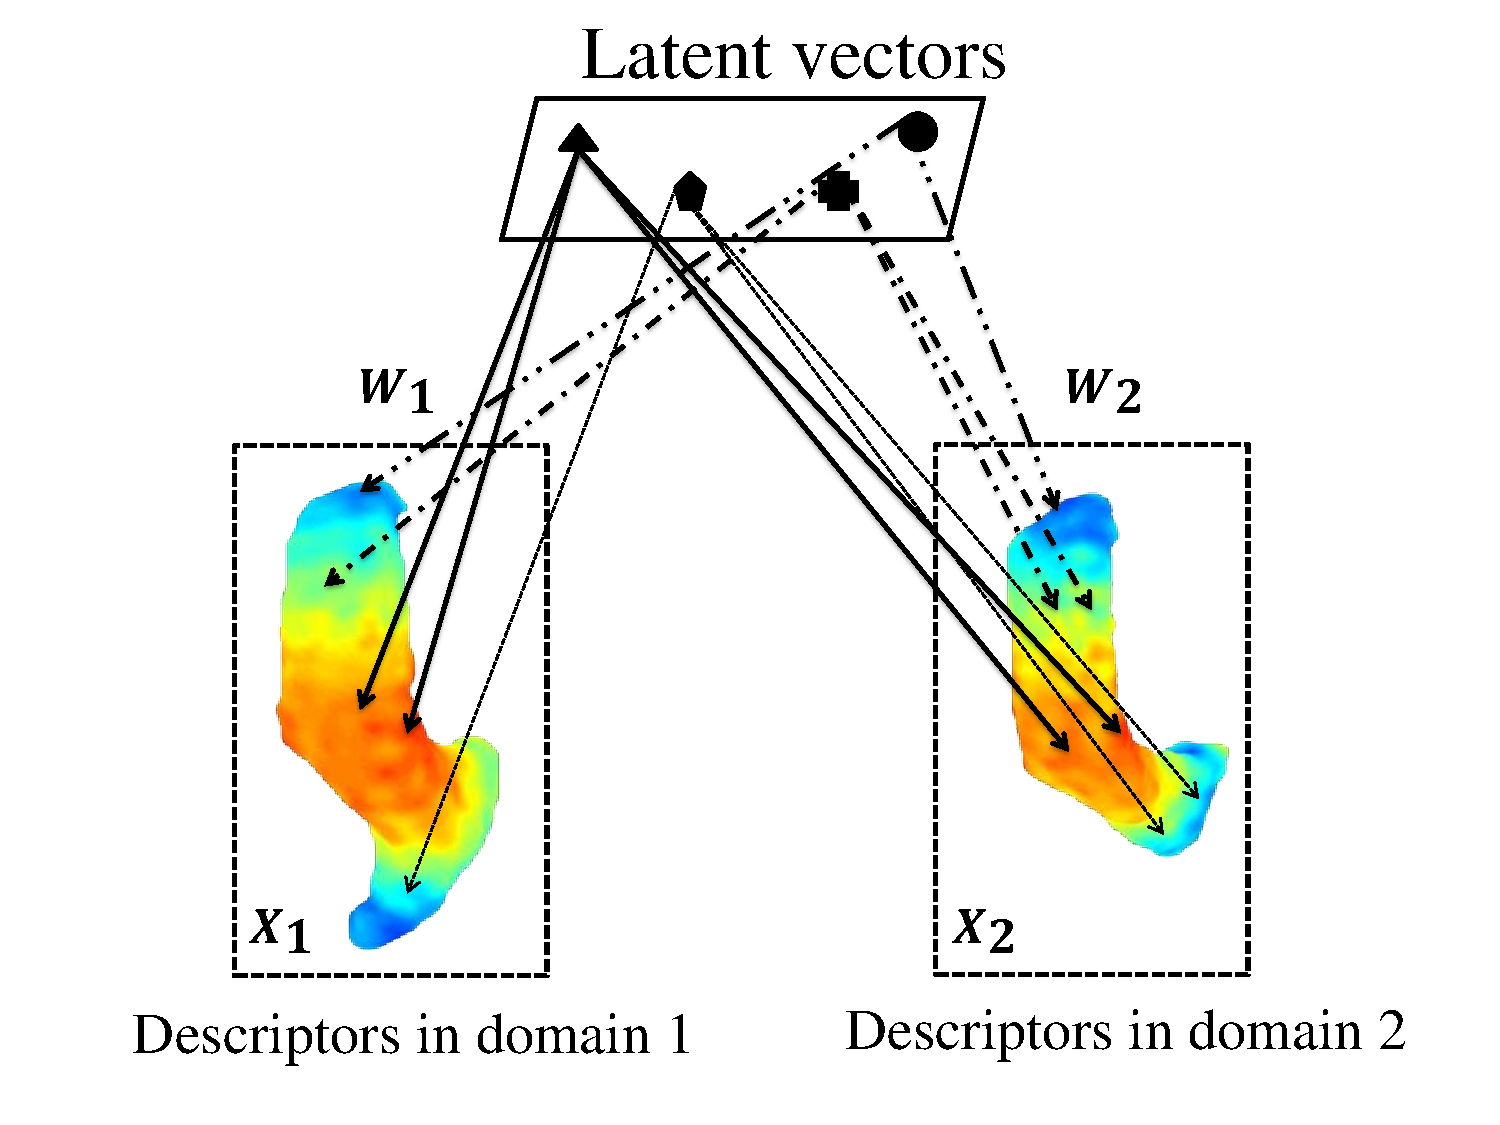
\includegraphics[width=0.6\textwidth]{img/pipelineGroupCorr}
\caption{Scheme for the groupwise correspondence method. The
  figure shows an example of establishing clusters of correspondences
  in two domains (left ventrals).}
\label{fig:pipeline}
\end{figure} 

In order to draw the cluster proportions, we use a stick-breaking process to generate mixture weights for a Dirichlet process with
concentration parameter $\gamma$ \cite{Iwata13} ($a$,$b$ and $r$ are the hyperparameters). The joint probability
of the data $\mathcal{X}$, and the cluster assignments
$\mathbf{S}=\left\{\left\{s_{dn}\right\}_{n=1}^{N_{d}}\right\}_{d=1}^{D}$
are given by
\begin{equation}
p\left(\boldsymbol{\Phi},\mathbf{S}|\boldsymbol{\mathcal{W}},a,b,r,\gamma\right)=
p\left(\mathbf{S}|\gamma\right)p\left(\boldsymbol{\Phi}|\mathbf{S},\boldsymbol{\mathcal{W}},a,b,r\right).
\label{eq:jointP}
\end{equation}


By marginalizing out the mixture weights $\boldsymbol{\theta}$, $p\left(\mathbf{S}|\gamma\right)$ becomes in
\begin{equation}
p\left(\mathbf{S}|\gamma\right) =\frac{\gamma^{J}\prod\limits_{j=1}^{J}{\left(N_{.j}-1\right)!}}{\gamma\left(\gamma+1\right)\dots\left(\gamma+N-1\right)},
\end{equation}
where $N=\sum\limits_{d=1}^{D}N_d$ is the total number of shape
descriptors, $N_{.j}$ represents the number of descriptors assigned to
the cluster $j$, and $J$ is the number of clusters that satisfies
$N_{.j}>0$. 

\subsection{The linear model (likelihood)}
By marginalizing out latent vectors $\mathbf{Z}$ and the
precision parameter $\alpha$, the second factor of \eqref{eq:llLinear} is
computed by

\begin{align}
p\left(\mathbf{X}|\Scluster,\WIn,a,b,r\right) &=  \int \int \prod_{d=1}^{D}\prod_{n=1}^{N_d}{\gD{\indobj|\projMatI \lvecsI}{\alpha^{-1}\eye}\catD{\alpha|a}{b}} \times \prod_{j=1}^{J}\gD{\lvecI|\mathbf{0}}{\left(\alpha r\right)^{-1}\eye}d\Z d\alpha  \notag \\
&=\int \int \prod_{d=1}^{D}\prod_{n=1}^{N_d}\left(\frac{\alpha}{2\pi}\right)^{M_d /2}\exp\left(-\frac{\alpha}{2}||\indobj-\projMatI\lvecsI||^2\right) \prod_{j=1}^{J}\left(\frac{\alpha r}{2\pi}\right)^{K/2} \notag \\
&\times \exp\left(-\frac{\alpha r}{2}||\lvecI||^2\right)\frac{b^a \alpha^{a-1}}{\gammaA}\exp\left(-b\alpha\right)d\Z d\alpha \notag\\
&=\frac{b^a}{\gammaA}\int \int \left(\frac{\alpha}{2\pi}\right)^{\sum_d M_d N_d /2}\exp\left(-\frac{\alpha}{2} \sum_{d=1}^{D}\sum_{n=1}^{N_d}||\indobj-\projMatI\lvecsI||^2\right)\left(\frac{\alpha r}{2\pi}\right)^{KJ/2} \notag \\
&\times \exp\left(-\frac{\alpha r}{2} \sum_{j=1}^{J}||\lvecI||^2\right)\exp\left(-b\alpha\right)\alpha^{a-1}d\Z d\alpha 
\label{eq:llnmlin}
\end{align}


Solving for the first exponential term

\begin{align}
\exp\left(-\frac{\alpha}{2} \sum_{d=1}^{D}\sum_{n=1}^{N_d}||\indobj-\projMatI\lvecsI||^2\right) &= \exp\Big(-\frac{\alpha}{2} \sum_{d=1}^{D}\sum_{n=1}^{N_d}\big[ \indobj^\top \indobj  \notag\\
&  - 2 \lvecsI ^\top \projMatI^\top \indobj + \lvecsI^\top \projMatI^\top \projMatI \lvecsI \big]\Big) \notag\\
%&=  \exp\Big(-\frac{\alpha}{2} \sum_{d=1}^{D}\sum_{n=1}^{N_d}\big[ \kernel{\indobj}{\indobj}  \notag\\
%&  - 2 \lvecs ^\top\underbrace{ \projMat^\top \phixnd }_{A}+ \lvecs^\top \underbrace{\projMat^T \projMat}_{B} \lvecs \big]\Big)
\label{eq:exp_XWzlin}
\end{align}

The equation in \eqref{eq:llnmlin} becomes

\begin{align}
p\left(\mathbf{X}|\Scluster,\WIn,a,b,r\right) &= \frac{b^a}{\gammaA}\int \int \left(\frac{\alpha}{2\pi}\right)^{\sum_d M_d N_d /2}\exp\Big(-\frac{\alpha}{2} \sum_{d=1}^{D}\sum_{n=1}^{N_d}\big[ \indobj^\top \indobj  \notag\\
&  - 2 \lvecsI ^\top \projMatI^\top \indobj + \lvecsI^\top \projMatI^\top \projMatI \lvecsI \big]\Big)\left(\frac{\alpha r}{2\pi}\right)^{KJ/2} \notag \\
&\times \exp\left(-\frac{\alpha r}{2} \sum_{j=1}^{J}\lvecI^\top\lvecI\right)\exp\left(-b\alpha\right)\alpha^{a-1}d\Z d\alpha.
\label{eq:llnmlin2}
\end{align}

The exponential terms in \eqref{eq:llnmlin2} becomes

\begin{align}
&\exp\Bigg(-\frac{\alpha}{2} \sum_{d=1}^{D}\sum_{n=1}^{N_d}\big[ \indobj^\top \indobj-2 \lvecsI ^\top \projMatI^\top \indobj + \lvecsI^\top \projMatI^\top \projMatI \lvecsI\big]-\frac{\alpha r}{2} \sum_{j=1}^{J}\lvecI^\top\lvecI -b\alpha\Bigg) = \notag\\
& \exp\Bigg(-\frac{\alpha}{2} \sum_{d=1}^{D}\sum_{n=1}^{N_d}\big[ \indobj^\top \indobj-b\alpha\Bigg)\exp\Bigg(-\frac{\alpha}{2} \sum_{d=1}^{D}\sum_{n=1}^{N_d}\big[ -2 \lvecsI ^\top \projMatI^\top \indobj+\lvecsI^\top \projMatI^\top \projMatI \lvecsI\big] \notag\\
&-\frac{\alpha r}{2} \sum_{j=1}^{J}\lvecI^\top\lvecI\Bigg) \label{eq:llKernelExp1lin}
\end{align}

By analyzing the $n$th objects that has the cluster assignment $j$ ($n:s_{dn}=j$), the second factor in \eqref{eq:llKernelExp1lin} becomes

\begin{align}
&\exp\Bigg(-\frac{\alpha}{2} \sum_{d=1}^{D}\sum_{n=1}^{N_d}\big[ -2 \lvecsI ^\top \projMatI^\top \indobj+\lvecsI^\top \projMatI^\top \projMatI \lvecsI \big] -\frac{\alpha r}{2} \sum_{j=1}^{J}\lvecI^\top\lvecI \Bigg) = \exp\Bigg(-\frac{\alpha}{2} \sum_{d=1}^{D}\sum_{n:s_{dn}\ne j}\big[  -2 \lvecsI ^\top \projMatI^\top \indobj\notag\\
&+ \lvecsI^\top \projMatI^\top \projMatI \lvecsI \big] \Bigg)\times \underbrace{\exp\Bigg(-\frac{\alpha}{2} \sum_{d=1}^{D}\sum_{n:s_{dn}=j}\big[ -2 \lvecsI ^\top \projMatI^\top \indobj+\lvecsI^\top \projMatI^\top \projMatI \lvecsI \big]-\frac{\alpha r}{2} \sum_{j=1}^{J}\lvecI^\top\lvecI\Bigg)}_{C} \notag\\
&=\exp\Bigg(-\frac{\alpha}{2} \sum_{d=1}^{D}\sum_{j=1}^J N_{dj}\big[ -2 \lvecI ^\top \projMatI^\top \indobj+\lvecI^\top \projMatI^\top \projMatI \lvecI \big]-\frac{\alpha r}{2} \sum_{j=1}^{J}\lvecI^\top\lvecI\Bigg) \notag\\
&=\exp\Bigg(-\frac{\alpha}{2} \sum_{d=1}^{D}\sum_{j=1}^J \big[ -2 \lvecI ^\top \projMatI^\top \sum_{n:s_{dn}=j}\indobj+\lvecI^\top N_{dj}\projMatI^\top \projMatI \lvecI \big]-\frac{\alpha r}{2} \sum_{j=1}^{J}\lvecI^\top\lvecI\Bigg) \notag \\
&=\exp\Bigg(-\frac{\alpha}{2}\sum_{j=1}^J \big[ -2 \lvecI ^\top  \sum_{d=1}^{D}\projMatI^\top \sum_{n:s_{dn}=j}\indobj+\lvecI^\top  \sum_{d=1}^{D} N_{dj}\projMatI^\top \projMatI \lvecI \big]-\frac{\alpha r}{2} \sum_{j=1}^{J}\lvecI^\top\lvecI\Bigg) \notag \\
&= \exp\Bigg(-\frac{\alpha}{2}\sum_{j=1}^J \big[ -2 \lvecI ^\top  \sum_{d=1}^{D}\projMatI^\top \sum_{n:s_{dn}=j}\indobj+\lvecI^\top  \sum_{d=1}^{D} N_{dj}\projMatI^\top \projMatI \lvecI + r\lvecI^\top\lvecI\big]\Bigg) \notag \\
&= \exp\Bigg(-\frac{\alpha}{2}\sum_{j=1}^J \big[ -2 \lvecI ^\top  \sum_{d=1}^{D}\projMatI^\top \sum_{n:s_{dn}=j}\indobj+\lvecI^\top  \left(\sum_{d=1}^{D} N_{dj}\projMatI^\top \projMatI + r\eye\right) \lvecI \big]\Bigg).
 \label{eq:llExp1lin}
\end{align}

By using the quadratic property

\begin{align}
-\frac{1}{2}\left(\mathbf{z}-\boldsymbol{\mu}\right)^\top \boldsymbol{C}^{-1} \left(\mathbf{z}-\boldsymbol{\mu}\right) = -\frac{1}{2}\left[\mathbf{z}^\top \boldsymbol{C}^{-1}\mathbf{z} -2\mathbf{z}^\top \boldsymbol{C}^{-1}\boldsymbol{\mu} + \boldsymbol{\mu}^\top\boldsymbol{C}^{-1}\boldsymbol{\mu}\right] \label{eq:quadlin},
\end{align}

where 

\begin{align}
\Cin^{-1} = \sum_{d=1}^{D} N_{dj}\projMatI^\top \projMatI + r\eye,
\end{align}

and

\begin{align}
-2\mathbf{z}^\top \boldsymbol{C}^{-1}\boldsymbol{\mu} &=  -2 \lvecI ^\top  \sum_{d=1}^{D}\projMatI^\top \sum_{n:s_{dn}=j}\indobj \notag \\
\muJ &= \Cin  \sum_{d=1}^{D}\projMatI^\top \sum_{n:s_{dn}=j}\indobj .
\end{align}

By completing the square as: $\textrm{arg} = \textrm{arg} + \frac{1}{2}\boldsymbol{\mu}^\top\boldsymbol{C^{-1}}\boldsymbol{\mu} -\frac{1}{2}\boldsymbol{\mu}^\top\boldsymbol{C^{-1}}\boldsymbol{\mu}$, the argument in \eqref{eq:llExp1lin} becomes

\begin{align}
&\exp\Bigg(-\frac{\alpha}{2}\sum_{j=1}^J \big[ -2 \lvecI ^\top  \sum_{d=1}^{D}\projMatI^\top \sum_{n:s_{dn}=j}\indobj+\lvecI^\top  \left(\sum_{d=1}^{D} N_{dj}\projMatI^\top \projMatI + r\eye\right) \lvecI \big]\Bigg) \notag\\ &= \exp\Bigg(-\frac{\alpha}{2}\Big[\sum_{j=1}^{J} \left(\lvecI-\muJ\right)^\top\Cin^{-1}\left(\lvecI-\muJ\right)\Big]\Bigg)
\exp\Bigg(-\frac{\alpha}{2}\sum_{j=1}^{J}\muJ^\top\Cin^{-1}\muJ\Bigg) \label{eq:expFinalKernlin}
\end{align}


Substituting \eqref{eq:expFinalKernlin} in \eqref{eq:llnmlin2} give us

\begin{align}
p\left(\mathbf{X}|\Scluster,\WIn,a,b,r\right)&=\frac{b^a}{\gammaA}\iint \left(\frac{\alpha}{2\pi}\right)^{\sum_d M_d N_d /2}\left(\frac{\alpha r}{2\pi}\right)^{KJ/2}\exp\Bigg(-\frac{\alpha}{2}\Big[\sum_{j=1}^{J} \left(\lvecI-\muJ\right)^\top\Cin^{-1}\left(\lvecI-\muJ\right)\Big]\Bigg)d\Z \notag\\
&\exp\Bigg(-\alpha\Bigg[\frac{1}{2} \sum_{d=1}^{D}\sum_{n=1}^{N_d}\indobj^\top \indobj  -\frac{1}{2}\sum_{j=1}^{J}\muJ^\top\Cin^{-1}\muJ +b \Bigg]\Bigg)\alpha^{a-1}d\alpha \label{eq:llFinalIntegralslin}
\end{align}

In equation \eqref{eq:llFinalIntegralslin}, factors related to $\Z$ are grouped together. We integrated out $\Z$ using

\begin{align}
\int \exp\left(-\frac{1}{2}\left(\lvecI-\muJ\right)^\top\left[\alpha^{-1}\Cin\right]^{-1}\left(\lvecI-\muJ\right)\right)d\lvecI = \left(2\pi\right)^{K/2}|\alpha^{-1}\Cin|^{1/2} = \left(2\pi\right)^{K/2}\alpha^{-K/2}|\Cin|^{1/2},
\end{align}

which is the normalization constant of $P$-dimensional Gaussian distribution. Since we have the sum over the number of correspondences (latent vectors), $K$, the above equation ranges for all of these clusters. The equation \eqref{eq:llFinalIntegralslin}, becomes

\begin{align}
p\left(\mathbf{X}|\Scluster,\WIn,a,b,r\right) &=\frac{b^a}{\gammaA}\int \left(\frac{\alpha}{2\pi}\right)^{\sum_d M_d N_d /2}\left(\frac{\alpha r}{2\pi}\right)^{KJ/2} \prod_{j=1}^{J}\Big[\left(2\pi\right)^{K/2}\alpha^{-K/2}|\Cin|^{1/2}\Big]
 \notag\\
&\exp\Bigg(-\alpha\Bigg[\frac{1}{2} \sum_{d=1}^{D}\sum_{n=1}^{N_d}\indobj^\top \indobj -\frac{1}{2}\sum_{j=1}^{J}\muJ^\top\Cin^{-1}\muJ +b \Bigg]\Bigg)\alpha^{a-1}d\alpha \\
&=\frac{b^a}{\gammaA}\int \left(\frac{\alpha}{2\pi}\right)^{\sum_d M_d N_d /2}\left(\frac{\alpha r}{2\pi}\right)^{KJ/2} \left(2\pi\right)^{KJ/2}\alpha^{-KJ/2}\prod_{j=1}^{J}|\Cin|^{1/2} \notag\\
&\exp\Bigg(-\alpha\Bigg[\frac{1}{2} \sum_{d=1}^{D}\sum_{n=1}^{N_d}\indobj^\top\indobj -\frac{1}{2}\sum_{j=1}^{J}\muJ^\top\Cin^{-1}\muJ +b \Bigg]\Bigg)\alpha^{a-1}d\alpha\label{eq:llFinalIntegralZlin}
\end{align}

The $\alpha$ parameter is integrated out by using the following normalization constant of a Gamma distribution 
\begin{align}
\int \alpha^{a'-1}\exp\left(-b\alpha\right)d\alpha = \frac{\Gamma\left(a'\right)}{b'^{a'}}.
\end{align}

Finally the likelihood is given by

\begin{align}
p\left(\mathbf{X}|\Scluster,\WIn,a,b,r\right) &=\left(2\pi\right)^{-\frac{\sum_d M_d N_d}{2}}r^{\frac{KJ}{2}}\frac{b^{a}}{b'^{a'}}\frac{\Gamma\left(a'\right)}{\Gamma\left(a\right)}\prod_{j=1}^{J}|\Cin|^{1/2},
\label{eq:llFinalIntegrallastlin}
\end{align}

Here,

\begin{align}
a'=a+{\frac{\Sigma_d M_d N_d}{2}}, \quad \quad b'=b+{\frac{1}{2}}\sum\limits_{d=1}^{D}\sum\limits_{n=1}^{N_d}{\mathbf{x}_{dn}^{\top}\mathbf{x}_{dn}}-{\frac{1}{2}}\sum\limits_{j=1}^{J}\boldsymbol{\mu}_j^\top \mathbf{C}_j^{-1}\boldsymbol{\mu}_j,
\end{align}
\begin{align}
\boldsymbol{\mu}_j =\mathbf{C}_j\sum\limits_{d=1}^{D}{\mathbf{W}_d^\top\sum\limits_{n:s_{dn}=j}{\mathbf{x}_{dn}}}, \quad \quad \mathbf{C}_{j}^{-1} =\sum\limits_{d=1}^{D}{N_{dj}\mathbf{W}_d^\top\mathbf{W}_d+r\mathbf{I}},
\end{align}

where $N_{dj}$ is the number of descriptors assigned to cluster $j$ in the shape $d$ (domain). 

\subsection{Inference for the Linear Model}

\subsubsection{M-Step Linear}

In the M-step, the projection matrices $\WIn$ are estimated by maximizing the logarithm of the joint likelihood \eqref{eq:jointP}. The gradient of the joint likelihood is computed by

\begin{align}
\frac{\partial \log p\left(\mathbf{X},\mathbf{S}|\WIn,a,b,r,\gamma\right)}{\partial\projMatI} =
\frac{\partial \log p\left(\mathbf{S}|\gamma\right)}{\partial\projMatI} + \frac{\partial \log p\left(\mathbf{X}|\mathbf{S},\boldsymbol{\mathbf{W}},a,b,r\right)}{\partial\projMatI},
\end{align}

Since the derivative of the first term in the above expression is zero, the expression becomes

\begin{align}
\frac{\partial \log p\left(\setX,\mathbf{S}|\WIn,a,b,r,\gamma\right)}{\partial\projMatI} &=
\frac{\partial \log p\left(\setX|\mathbf{S},\WIn,a,b,r\right)}{\partial\projMatI} = \frac{\partial \log \Big[\left(2\pi\right)^{-\frac{\sum_d M_d N_d}{2}}r^{\frac{JK}{2}}\frac{b^{a}}{b'^{a'}}\frac{\Gamma\left(a'\right)}{\Gamma\left(a\right)}\prod_{j=1}^{J}|\Cin|^{1/2}\Big]}{\partial\projMat},\notag\\
&= \frac{\partial \log \Big[\frac{cte}{b'^{a'}} \prod_{j=1}^{J}|\Cin|^{1/2}\Big]}{\partial\projMatI}\notag,\\
& = -\frac{a'}{b'}\frac{\partial b'}{\dWjIn}+\frac{1}{2}\sum_{j=1}^{J}\frac{\partial \log |\Cin|}{\dWjIn}+0 , \notag \\
& =  -\frac{a'}{b'}\frac{\partial b'}{\dWjIn}+\frac{1}{2}\sum_{j=1}^{J} \operatorname{tr}\left(\Cin^{-1}\frac{\partial \Cin}{\dWjIn}\right)
%\label{eq:derivativeW1}
\end{align}

where

\begin{align}
\frac{\partial b'}{\dWjIn} = \frac{\partial}{\dWjIn}\Big[ \frac{1}{2} \sum_{d=1}^{D}\sum_{n=1}^{N_d}\indobj^\top\indobj -\frac{1}{2}\sum_{j=1}^{J}\muJ^\top\Cin^{-1}\muJ +b \Big],
\end{align}

Here the second factor of the argument is the only which depends on $\projMat$.
%\C\sum\limits_{d=1}^{D}{\sum\limits_{n:s_{dn}=j}\kawx}
\begin{align}
\frac{\partial b'}{\dWjIn} &= \frac{\partial}{\dWjIn}\Big[-\frac{1}{2}\sum_{j=1}^{J}\muJ^\top\Cin^{-1}\muJ \Big] \notag \\
&=-\frac{1}{2}\sum_{j=1}^{J}\frac{\partial}{\dWjIn}\Big[\muJ^\top\Cin^{-1}\muJ \Big] =-\frac{1}{2}\sum_{j=1}^{J}\tr\left(\frac{\partial}{\dWjIn}\Big[\muJ^\top\Cin^{-1}\muJ \Big]\right) \notag \\
&=-\frac{1}{2}\sum_{j=1}^{J}\tr\left(\frac{\partial \muJ^\top}{\dWjIn}\Cin^{-1}\muJ + \muJ^\top\left(\frac{\partial \Cin^{-1}}{\dWjIn}\muJ+\Cin^{-1}\frac{\partial \muJ}{\dWjIn}\right)\right) \notag \\
& = -\frac{1}{2}\sum_{j=1}^{J} \tr\left(\partial \muJ^\top\Cin^{-1}\muJ\right) + \tr\left( \muJ^\top\partial\Cin^{-1}\muJ\right) + \tr\left( \muJ^\top\Cin^{-1}\partial\muJ\right),
\end{align}

by applying trace properties (transpose elements)

\begin{align}
\frac{\partial b'}{\dWjIn} &= -\frac{1}{2}\sum_{j=1}^{J} \tr\left(\partial \muJ^\top\Cin^{-1}\muJ\right) + \tr\left( \muJ^\top\partial\Cin^{-1}\muJ\right) + \tr\left( \muJ^\top\Cin^{-1}\partial\muJ\right) \notag \\
&=  -\frac{1}{2}\sum_{j=1}^{J} \tr\left( \muJ^\top\Cin^{-1}\partial\muJ\right) + \tr\left( \muJ^\top\partial\Cin^{-1}\muJ\right) + \tr\left( \muJ^\top\Cin^{-1}\partial\muJ\right) \notag \\
&= -\frac{1}{2}\sum_{j=1}^{J} \tr\left( \muJ^\top\partial\Cin^{-1}\muJ\right) + 2\tr\left( \muJ^\top\Cin^{-1}\partial\muJ\right) \notag\\
&=  \underbrace{-\sum_{j=1}^{J}\tr\left( \muJ^\top\Cin^{-1}\partial\muJ\right)}_{A} \underbrace{-\frac{1}{2}\sum_{j=1}^{J} \tr\left( \muJ^\top\partial\Cin^{-1}\muJ\right)}_{B} 
\end{align}

First, for the B part we have:

% % % % % % % % % % % % % % % % % % % % % % % % % % %


\begin{align}
-\frac{1}{2}\sum_{j=1}^{J} \tr\left( \muJ^\top\partial\Cin^{-1}\muJ\right) &= -\frac{1}{2}\sum_{j=1}^{J} \tr\left( \muJ^\top\partial\left[\sum_{d=1}^{D}N_{dj}\projMatI^\top\projMatI+r\mathbf{I}\right]\muJ\right) \notag \\
&=  -\frac{1}{2}\sum_{j=1}^{J} \tr\left( \muJ^\top\left[N_{dj}\left(\partial\projMatI^\top\projMatI+\projMatI^\top\partial\projMatI\right)\right]\muJ\right) \notag \\
&=  -\frac{1}{2}\sum_{j=1}^{J} \left[N_{dj}\tr\left( \muJ^\top\partial\projMatI^\top\projMatI\muJ\right)+N_{dj}\tr\left(\muJ^\top\projMatI^\top\partial\projMatI\muJ\right)\right] \notag \\
&=  -\frac{1}{2}\sum_{j=1}^{J} \left[N_{dj}\tr\left( \left(\muJ^\top\partial\projMatI^\top\projMatI\muJ\right)^\top\right)+N_{dj}\tr\left(\muJ\muJ^\top\projMatI^\top\partial\projMatI\right)\right] \notag\\
&=  -\frac{1}{2}\sum_{j=1}^{J} \left[N_{dj}\tr\left( \muJ\muJ^\top\projMatI^\top\partial\projMatI\muJ\right)+N_{dj}\tr\left(\muJ\muJ^\top\projMatI^\top\partial\projMatI\right)\right] \notag\\
&=  -\sum_{j=1}^{J} N_{dj}\tr\left( \muJ\muJ^\top\projMatI^\top\partial\projMatI\right).
\label{eq:partBLinearMstep}
\end{align}


By using derivatives properties for trace forms as 
\begin{align}
\frac{\partial \tr\left[F\left(\mathbf{X}\right)\right]}{\partial \mathbf{X}} = f\left(\mathbf{X}\right)^\top,
\end{align}

where $f\left(\cdot\right)$ is the scalar derivative of $F\left(\cdot\right)$, the equation \eqref{eq:partBLinearMstep} becomes

\begin{align}
-\frac{1}{2}\sum_{j=1}^{J} \tr\left( \muJ^\top\partial\Cin^{-1}\muJ\right) &= -\sum_{j=1}^{J} N_{dj}\left( \muJ\muJ^\top\projMatI^\top\right)^\top =  -\sum_{j=1}^{J} N_{dj} \projMatI \muJ\muJ^\top.
\end{align}

Besides, for the A part we have:

\begin{align}
-\sum_{j=1}^{J}\tr\left( \muJ^\top\Cin^{-1}\partial\muJ\right) \rightarrow \frac{\partial \muJ}{\partial \projMatI} = \frac{\partial}{\partial \projMatI}\left[\Cin\sum_{d=1}^{D}\projMatI^\top\sum_{n:s_{dn}=j}\indobj\right].
\end{align}

The derivative for $\muJ$ is given by

\begin{align}
\frac{\partial \muJ}{\partial \projMatI} &= \underbrace{\partial\Cin\left(\sum_{d=1}^{D}\projMatI^\top\sum_{n:s_{dn}=j}\indobj\right)}_{C} + \underbrace{\Cin\partial\left(\sum_{d=1}^{D}\projMatI^\top\sum_{n:s_{dn}=j}\indobj\right)}_{D} 
\end{align}

For the $C$ part, we have

\begin{align}
\partial\Cin\left(\sum_{d=1}^{D}\projMatI^\top\sum_{n:s_{dn}=j}\indobj\right) &= \frac{\partial}{\partial \projMatI}\left[\left(\sum_{d=1}^{D}N_{dj}\projMatI^\top\projMatI+r\mathbf{I}\right)^{-1}\right]\left(\sum_{d=1}^{D}\projMatI^\top\sum_{n:s_{dn}=j}\indobj\right) \notag \\
&= -\Cin \frac{\partial}{\partial \projMatI}\left[\sum_{d=1}^{D}N_{dj}\projMatI^\top\projMatI+r\mathbf{I}\right]\Cin\sum_{d=1}^{D}\projMatI^\top\sum_{n:s_{dn}=j}\indobj \notag\\
&=-\Cin\left(N_{dj}\left[\partial\projMatI^\top\projMatI+\projMatI^\top\partial\projMatI\right]\right)\muJ.
\end{align}

The $D$ part is computed as

\begin{align}
\Cin\partial\left(\sum_{d=1}^{D}\projMatI^\top\sum_{n:s_{dn}=j}\indobj\right) = \Cin\partial\projMatI^\top\sum_{n:s_{dn}=j}\indobj.
\end{align}

Then the $A$ part becomes,

\begin{align}
-\sum_{j=1}^{J}\tr\left( \muJ^\top\Cin^{-1}\partial\muJ\right) &=-\sum_{j=1}^{J}\tr\left( \muJ^\top\Cin^{-1}\left[-\Cin\left(N_{dj}\left[\partial\projMatI^\top\projMatI+\projMatI^\top\partial\projMatI\right]\right)\muJ+\Cin\partial\projMatI^\top\sum_{n:s_{dn}=j}\indobj\right]\right) \notag \\
&= \sum_{j=1}^{J}N_{dj}\tr\left(\muJ^\top\Cin^{-1}\Cin\left(\partial\projMatI^\top\projMatI\right)\muJ\right) +  \sum_{j=1}^{J}N_{dj}\tr\left(\muJ^\top\Cin^{-1}\Cin\left(\projMatI^\top\partial\projMatI\right)\muJ\right) \notag\\
&-\sum_{j=1}^{J}\tr\left(\muJ^\top\Cin^{-1}\Cin\partial\projMatI^\top\sum_{n:s_{dn}=j}\indobj\right) \notag \\
&= \sum_{j=1}^{J}N_{dj}\tr\left(\muJ^\top\partial\projMatI^\top\projMatI\muJ\right) +  \sum_{j=1}^{J}N_{dj}\tr\left(\muJ^\top\projMatI^\top\partial\projMatI\muJ\right) \notag\\
&-\sum_{j=1}^{J}\tr\left(\muJ^\top\partial\projMatI^\top\sum_{n:s_{dn}=j}\indobj\right) \notag \\
&= \sum_{j=1}^{J}N_{dj}\tr\left(\left(\muJ^\top\partial\projMatI^\top\projMatI\muJ\right)^\top\right) +  \sum_{j=1}^{J}N_{dj}\tr\left(\muJ\muJ^\top\projMatI^\top\partial\projMatI\right) \notag\\
&-\sum_{j=1}^{J}\tr\left(\left(\muJ^\top\partial\projMatI^\top\sum_{n:s_{dn}=j}\indobj\right)^\top\right) \notag \\
&= \sum_{j=1}^{J}N_{dj}\tr\left(\muJ^\top\projMatI^\top\partial\projMatI\muJ\right) +  \sum_{j=1}^{J}N_{dj}\tr\left(\muJ\muJ^\top\projMatI^\top\partial\projMatI\right) \notag\\
&-\sum_{j=1}^{J}\tr\left(\sum_{n:s_{dn}=j}\indobj^\top\partial\projMatI\muJ\right) \notag \\
&= \sum_{j=1}^{J}N_{dj}\tr\left(\muJ\muJ^\top\projMatI^\top\partial\projMatI\right) +  \sum_{j=1}^{J}N_{dj}\tr\left(\muJ\muJ^\top\projMatI^\top\partial\projMatI\right) \notag\\
&-\sum_{j=1}^{J}\tr\left(\muJ\sum_{n:s_{dn}=j}\indobj^\top\partial\projMatI\right) \notag \\
&= 2\sum_{j=1}^{J}N_{dj}\tr\left(\muJ\muJ^\top\projMatI^\top\partial\projMatI\right)-\sum_{j=1}^{J}\tr\left(\muJ\sum_{n:s_{dn}=j}\indobj^\top\partial\projMatI\right) .
\end{align}


By using the derivatives properties for trace forms described above, we have

\begin{align}
-\sum_{j=1}^{J}\tr\left( \muJ^\top\Cin^{-1}\partial\muJ\right) &= 2\sum_{j=1}^{J}N_{dj}\left(\muJ\muJ^\top\projMatI^\top\right)^\top-\sum_{j=1}^{J}\left(\muJ\sum_{n:s_{dn}=j}\indobj^\top\right)^\top \notag \\
&= 2\sum_{j=1}^{J}N_{dj}\projMatI\muJ\muJ^\top - \sum_{j=1}^{J}\sum_{n:s_{dn}=j}\indobj \muJ^\top .
\end{align}

Finally 

\begin{align}
\frac{\partial b'}{\dWjIn} &= 2\sum_{j=1}^{J}N_{dj}\projMatI\muJ\muJ^\top - \sum_{j=1}^{J}\sum_{n:s_{dn}=j}\indobj \muJ^\top -  -\sum_{j=1}^{J} N_{dj} \projMatI \muJ\muJ^\top \notag \\
&= \sum_{j=1}^{J}N_{dj}\projMatI\muJ\muJ^\top - \sum_{j=1}^{J}\sum_{n:s_{dn}=j}\indobj \muJ^\top \notag \\
&= \sum_{j=1}^{J}\left\{N_{dj}\projMatI\muJ\muJ^\top - \sum_{n:s_{dn}=j}\indobj \muJ^\top\right\}.
\end{align}

For the part $B$,

\begin{align}
\frac{1}{2}\sum_{j=1}^{J} \operatorname{Tr}\left(\Cin^{-1}\frac{\partial \Cin}{\dWjIn}\right) &= \frac{1}{2}\sum_{j=1}^{J} \operatorname{tr}\left(\Cin^{-1}\left(-\Cin\left(N_{dj}\left[\partial\projMatI^\top\projMatI+\projMatI^\top\partial\projMatI\right]\right)\Cin\right)\right) \notag \\
&= -\frac{1}{2}\sum_{j=1}^{J}N_{dj}\operatorname{tr}\left(\Cin^{-1}\Cin\left[\partial\projMatI^\top\projMatI+\projMatI^\top\partial\projMatI\right]\Cin\right) \notag \\
&= -\frac{1}{2}\sum_{j=1}^{J}N_{dj}\operatorname{tr}\left(\Cin^{-1}\Cin\left[\partial\projMatI^\top\projMatI+\projMatI^\top\partial\projMatI\right]\Cin\right) \notag \\
&= -\frac{1}{2}\sum_{j=1}^{J}N_{dj}\operatorname{tr}\left(\partial\projMatI^\top\projMatI\Cin\right) -\frac{1}{2}\sum_{j=1}^{J}N_{dj}\operatorname{tr}\left(\projMatI^\top\partial\projMatI\Cin\right)\notag \\
&= -\frac{1}{2}\sum_{j=1}^{J}N_{dj}\operatorname{tr}\left(\left(\partial\projMatI^\top\projMatI\Cin\right)^\top\right) -\frac{1}{2}\sum_{j=1}^{J}N_{dj}\operatorname{tr}\left(\Cin\projMatI^\top\partial\projMatI\right)\notag \\
&= -\frac{1}{2}\sum_{j=1}^{J}N_{dj}\operatorname{tr}\left(\Cin\projMatI^\top\partial\projMatI\right) -\frac{1}{2}\sum_{j=1}^{J}N_{dj}\operatorname{tr}\left(\Cin\projMatI^\top\partial\projMatI\right)\notag \\
&=-\sum_{j=1}^{J}N_{dj}\operatorname{tr}\left(\Cin\projMatI^\top\partial\projMatI\right)= -\sum_{j=1}^{J}N_{dj}\projMatI\Cin.
\end{align}

Finally the derivative of the log-likelihood is computed as

\begin{align}
\frac{\partial \log p\left(\mathbf{X},\mathbf{S}|\WIn,a,b,r,\gamma\right)}{\partial\projMatI}  &=  -\frac{a'}{b'}\frac{\partial b'}{\dWjIn}+\frac{1}{2}\sum_{j=1}^{J} \operatorname{tr}\left(\Cin^{-1}\frac{\partial \Cin}{\dWjIn}\right) \notag \\
&=  -\frac{a'}{b'}\left[\sum_{j=1}^{J}\left\{N_{dj}\projMatI\muJ\muJ^\top - \sum_{n:s_{dn}=j}\indobj \muJ^\top\right\}\right] -\sum_{j=1}^{J}N_{dj}\projMatI\Cin.
\end{align}

We can obtain the projection matrices that maximize the joint likelihood analytically as follows,

\begin{align}
\projMatI =  -\frac{a'}{b'}\left(\sum_{j=1}^{J}{\sum_{n:s_{dn}=j}\indobj \muJ^\top}\right)\left(\sum_{j=1}^{J}{N_{dj}\Cin+\frac{a'}{b'}N_{dj}\muJ\muJ^\top} \right)^{-1}.
\end{align}

% % % % % % % % % % % % % % % % % % % % % % % % % % % % % % %5
\subsection{Likelihood for the non-linear model}

For the non-linear model, we give the derivation of the likelihood in \eqref{eq:llNLmodel}, in which latent vectors $\Z$ and precision parameter $\alpha$ are analytically integrated out. To this end, we use two mappings functions $\phixnd$ and $\phiwld{j}$, in order to represent our observations in the Hilbert space. First let us define the following expressions:

Let us define the projection matrix $\projMat$ in $\mathcal{H}$ as

\begin{align}
\projMat =
\left(\begin{matrix}
   \phiwldI{1}{1} & \phiwldI{2}{1} & \cdots& \phiwldI{P}{1}  \\
   \phiwldI{1}{2} & \phiwldI{2}{2} &\cdots& \phiwldI{P}{2}  \\
   \vdots  & \vdots  & \ddots & \vdots  \\
   \phiwldI{1}{L_d} & \phiwldI{2}{L_d} &\cdots& \phiwldI{P}{L_d}
   \end{matrix} \right)
\end{align}



\begin{align}
p\left(\boldsymbol{\Phi}|\Scluster,\W,a,b,r\right) &=  \int \int \prod_{d=1}^{D}\prod_{n=1}^{N_d}{\gD{\phixnd|\projMat \lvecs}{\alpha^{-1}\eye}\catD{\alpha|a}{b}} \times \prod_{j=1}^{Q}\gD{\lvec|\mathbf{0}}{\left(\alpha r\right)^{-1}\eye}d\Z d\alpha  \notag \\
&=\int \int \prod_{d=1}^{D}\prod_{n=1}^{N_d}\left(\frac{\alpha}{2\pi}\right)^{L_d /2}\exp\left(-\frac{\alpha}{2}||\phixnd-\projMat\lvecs||^2\right) \prod_{j=1}^{Q}\left(\frac{\alpha r}{2\pi}\right)^{P/2} \notag \\
&\times \exp\left(-\frac{\alpha r}{2}||\lvec||^2\right)\frac{b^a \alpha^{a-1}}{\gammaA}\exp\left(-b\alpha\right)d\Z d\alpha \notag\\
&=\frac{b^a}{\gammaA}\int \int \left(\frac{\alpha}{2\pi}\right)^{\sum_d L_d N_d /2}\exp\left(-\frac{\alpha}{2} \sum_{d=1}^{D}\sum_{n=1}^{N_d}||\phixnd-\projMat\lvecs||^2\right)\left(\frac{\alpha r}{2\pi}\right)^{PQ/2} \notag \\
&\times \exp\left(-\frac{\alpha r}{2} \sum_{j=1}^{Q}||\lvec||^2\right)\exp\left(-b\alpha\right)\alpha^{a-1}d\Z d\alpha 
\label{eq:llnm}
\end{align}

Solving for the first exponential term

\begin{align}
\exp\left(-\frac{\alpha}{2} \sum_{d=1}^{D}\sum_{n=1}^{N_d}||\phixnd-\projMat\lvecs||^2\right) &= \exp\Big(-\frac{\alpha}{2} \sum_{d=1}^{D}\sum_{n=1}^{N_d}\big[ \phixnd^\top \phixnd  \notag\\
&  - 2 \lvecs ^\top \projMat^\top \phixnd + \lvecs^\top \projMat^\top \projMat \lvecs \big]\Big) \notag\\
%&=  \exp\Big(-\frac{\alpha}{2} \sum_{d=1}^{D}\sum_{n=1}^{N_d}\big[ \kernel{\indobj}{\indobj}  \notag\\
%&  - 2 \lvecs ^\top \projMat^\top \phixnd+ \lvecs^\top \projMat^\top \projMat \lvecs \big]\Big)
\label{eq:exp_XWz}
\end{align}

The equation in \eqref{eq:llnm} becomes

\begin{align}
p\left(\boldsymbol{\Phi}|\Scluster,\W,a,b,r\right) &= \frac{b^a}{\gammaA}\int \int \left(\frac{\alpha}{2\pi}\right)^{\sum_d L_d N_d /2}\exp\Big(-\frac{\alpha}{2} \sum_{d=1}^{D}\sum_{n=1}^{N_d}\big[  \phixnd^\top \phixnd   \notag\\
&  - 2 \lvecs ^\top \projMat^\top \phixnd + \lvecs^\top \projMat^\top \projMat \lvecs \big]\Big)\left(\frac{\alpha r}{2\pi}\right)^{PQ/2} \notag \\
&\times \exp\left(-\frac{\alpha r}{2} \sum_{j=1}^{Q}\lvec^\top\lvec\right)\exp\left(-b\alpha\right)\alpha^{a-1}d\Z d\alpha.
\label{eq:llnm2}
\end{align}

The exponential terms in \eqref{eq:llnmlin2} becomes

\begin{align}
&\exp\Bigg(-\frac{\alpha}{2} \sum_{d=1}^{D}\sum_{n=1}^{N_d}\big[ \phixnd^\top \phixnd- 2 \lvecs ^\top \projMat^\top \phixnd + \lvecs^\top \projMat^\top \projMat \lvecs\big]-\frac{\alpha r}{2} \sum_{j=1}^{Q}\lvec^\top\lvec -b\alpha\Bigg) = \notag\\
& \exp\Bigg(-\frac{\alpha}{2} \sum_{d=1}^{D}\sum_{n=1}^{N_d}\big[ \phixnd^\top \phixnd-b\alpha\Bigg)\exp\Bigg(-\frac{\alpha}{2} \sum_{d=1}^{D}\sum_{n=1}^{N_d}\big[ -2 \lvecs ^\top \projMat^\top \phixnd + \lvecs^\top \projMat^\top \projMat \lvecs\big] \notag\\
&-\frac{\alpha r}{2} \sum_{j=1}^{Q}\lvec^\top\lvec\Bigg) 
\label{eq:llKernelExp1nm}
\end{align}

By analyzing the $n$th objects that has the cluster assignment $j$ ($n:s_{dn}=j$), the second factor in \eqref{eq:llKernelExp1nm} becomes

\begin{align}
&\exp\Bigg(-\frac{\alpha}{2} \sum_{d=1}^{D}\sum_{n=1}^{N_d}\big[ -2 \lvecs ^\top \projMat^\top \phixnd +\lvecs^\top \projMat^\top \projMat \lvecs \big] -\frac{\alpha r}{2} \sum_{j=1}^{Q}\lvec^\top\lvec \Bigg) \notag \\
&= \exp\Bigg(-\frac{\alpha}{2} \sum_{d=1}^{D}\sum_{n:s_{dn}\ne j}\big[  -2 \lvecs ^\top \projMat^\top \phixnd+ \lvecs^\top \projMat^\top \projMat \lvecs \big] \Bigg) \notag\\
&\times \exp\Bigg(-\frac{\alpha}{2} \sum_{d=1}^{D}\sum_{n:s_{dn}=j}\big[ -2 \lvecs ^\top \projMat^\top \phixnd+\lvecs^\top \projMat^\top \projMat \lvecs \big]-\frac{\alpha r}{2} \sum_{j=1}^{Q}\lvec^\top\lvec\Bigg) \notag\\
&=\exp\Bigg(-\frac{\alpha}{2} \sum_{d=1}^{D}\sum_{j=1}^Q N_{dj}\big[ -2 \lvec ^\top \projMat^\top \phixnd+\lvec^\top \projMat^\top \projMat \lvec \big]-\frac{\alpha r}{2} \sum_{j=1}^{J}\lvec^\top\lvec\Bigg) \notag\\
&=\exp\Bigg(-\frac{\alpha}{2} \sum_{d=1}^{D}\sum_{j=1}^Q \big[ -2 \lvec ^\top \projMat^\top \sum_{n:s_{dn}=j}\phixnd+\lvec^\top N_{dj}\projMatI^\top \projMat \lvec \big]-\frac{\alpha r}{2} \sum_{j=1}^{Q}\lvec^\top\lvec\Bigg) \notag \\
&=\exp\Bigg(-\frac{\alpha}{2}\sum_{j=1}^Q \big[ -2 \lvec^\top  \sum_{d=1}^{D}\projMat^\top \sum_{n:s_{dn}=j}\phixnd+\lvec^\top  \sum_{d=1}^{D} N_{dj}\projMat^\top \projMat \lvec \big]-\frac{\alpha r}{2} \sum_{j=1}^{Q}\lvec^\top\lvec\Bigg) \notag \\
&= \exp\Bigg(-\frac{\alpha}{2}\sum_{j=1}^Q \big[ -2 \lvec ^\top  \sum_{d=1}^{D}\projMat^\top \sum_{n:s_{dn}=j}\phixnd+\lvec^\top  \sum_{d=1}^{D} N_{dj}\projMat^\top \projMat \lvec + r\lvec^\top\lvec\big]\Bigg) \notag \\
&= \exp\Bigg(-\frac{\alpha}{2}\sum_{j=1}^Q \big[ -2 \lvec ^\top  \sum_{d=1}^{D}\projMat^\top \sum_{n:s_{dn}=j}\phixnd+\lvec^\top  \left(\sum_{d=1}^{D} N_{dj}\projMat^\top \projMat + r\eye\right) \lvec \big]\Bigg),
 \label{eq:llExp1nm}
\end{align}

where $N_{dj}$ is the number of objects assigned to cluster $j$ in de domain $d$. By using the quadratic property

\begin{align}
-\frac{1}{2}\left(\mathbf{z}-\boldsymbol{\mu}\right)^\top \boldsymbol{\Lambda}^{-1} \left(\mathbf{z}-\boldsymbol{\mu}\right) = -\frac{1}{2}\left[\mathbf{z}^\top \boldsymbol{\Lambda}^{-1}\mathbf{z} -2\mathbf{z}^\top \boldsymbol{\Lambda}^{-1}\boldsymbol{\mu} + \boldsymbol{\mu}^\top\boldsymbol{\Lambda}^{-1}\boldsymbol{\mu}\right] \label{eq:quadnm},
\end{align}

where 

\begin{align}
\C^{-1} = \sum_{d=1}^{D} N_{dj}\underbrace{\projMat^\top \projMat}_{A} + r\eye,
\end{align}

and

\begin{align}
-2\mathbf{z}^\top \boldsymbol{\Lambda}^{-1}\boldsymbol{\mu} &=  -2 \lvec^\top  \sum_{d=1}^{D}\projMat^\top \sum_{n:s_{dn}=j}\phixnd \notag \\
\muJ &= \C  \sum_{d=1}^{D}\projMat^\top \sum_{n:s_{dn}=j}\phixnd \notag \\
\muJ &= \C  \sum_{d=1}^{D} \sum_{n:s_{dn}=j}\underbrace{ \projMat^\top\phixnd}_{B}.
\end{align}

We can rewrite the expression in $A$ by placing a given kernel for $\projMat$

\begin{align}
 \projMat^\top \projMat 
% &= 
% \left[
%  \begin{matrix}
%     \phiwldI{1}{1} & \phiwldI{1}{2} & \cdots& \phiwldI{1}{L_d}  \\
%     \phiwldI{2}{1} & \phiwldI{2}{2} &\cdots& \phiwldI{2}{L_d}  \\
%     \vdots  & \vdots  & \ddots & \vdots  \\
%     \phiwldI{P}{1} & \phiwldI{P}{L_d} &\cdots& \phiwldI{P}{L_d}
%     \end{matrix}
%  \right]\times
% \left[
% \begin{matrix}
%    \phiwldI{1}{1} & \phiwldI{2}{1} & \cdots& \phiwldI{P}{1}  \\
%    \phiwldI{1}{2} & \phiwldI{2}{2} &\cdots& \phiwldI{P}{2}  \\
%    \vdots  & \vdots  & \ddots & \vdots  \\
%    \phiwldI{1}{L_d} & \phiwldI{2}{L_d} &\cdots& \phiwldI{P}{L_d}
%    \end{matrix}
% \right] \notag\\
  &=\left[
  \begin{matrix}
  \phiwld{1}^\top\phiwld{1}& \phiwld{1}^\top\phiwld{2} & \cdots & \phiwld{1}^\top\phiwld{P} \\
  \phiwld{2}^\top\phiwld{1}& \phiwld{2}^\top\phiwld{2} & \cdots & \phiwld{2}^\top\phiwld{P} \\
  \vdots  & \vdots  & \ddots & \vdots  \\
  \phiwld{P}^\top\phiwld{1}& \phiwld{P}^\top\phiwld{2} & \cdots & \phiwld{P}^\top\phiwld{P}
  \end{matrix}\right] \notag\\
  &=
  \left[ \begin{matrix}
   \kernelww{1}{1} & \kernelww{1}{2} & \cdots & \kernelww{1}{P}\\
   \kernelww{2}{1} & \kernelww{2}{2} & \cdots & \kernelww{2}{P}\\
   \vdots  & \vdots  & \ddots & \vdots  \\
   \kernelww{P}{1} & \kernelww{P}{2} & \cdots & \kernelww{P}{P}\\
   \end{matrix}\right] = \mathbf{\hat{K}}_{d}. \label{eq:Kp}
\end{align}


We can rewrite the expression in $B$ by placing a given kernel of the form

\begin{align}
 \projMat^\top \phixnd = 
 \left[ \begin{matrix}
	\phiwld{1}^\top\phixnd\\
  \phiwld{2}^\top\phixnd\\
  \vdots\\
  \phiwld{P}^\top\phixnd\\
  \end{matrix}\right]
= 
\left[ \begin{matrix}
 \kernelwx{1}\\
 \kernelwx{2}\\
 \vdots\\
 \kernelwx{P} 
 \end{matrix}\right] = \mathbf{\hat{k}}_d, \label{eq:kp}
\end{align}

where $\kawx$ represents the kernel evaluated in the $\indobj$ objects that has the cluster assignment $j$.\\

By completing the square as: $\textrm{arg} = \textrm{arg} + \frac{1}{2}\boldsymbol{\mu}^\top\boldsymbol{\C^{-1}}\boldsymbol{\mu} -\frac{1}{2}\boldsymbol{\mu}^\top\boldsymbol{\C^{-1}}\boldsymbol{\mu}$, the argument in \eqref{eq:llExp1lin} becomes

\begin{align}
&\exp\Bigg(-\frac{\alpha}{2}\sum_{j=1}^Q \big[ -2 \lvec ^\top  \sum_{d=1}^{D} \sum_{n:s_{dn}=j}\kawx+\lvec^\top  \left(\sum_{d=1}^{D} N_{dj}\Kaww + r\eye\right) \lvec \big]\Bigg) \notag\\ &= \exp\Bigg(-\frac{\alpha}{2}\Big[\sum_{j=1}^{Q} \left(\lvec-\muJ\right)^\top\C^{-1}\left(\lvec-\muJ\right)\Big]\Bigg)
\exp\Bigg(-\frac{\alpha}{2}\sum_{j=1}^{Q}\muJ^\top\C^{-1}\muJ\Bigg) \label{eq:expFinalKernnm}
\end{align}


Substituting \eqref{eq:expFinalKernnm} in \eqref{eq:llnm2} give us

\begin{align}
p\left(\boldsymbol{\Phi}|\Scluster,\W,a,b,r\right)&=\frac{b^a}{\gammaA}\iint \left(\frac{\alpha}{2\pi}\right)^{\sum_d L_d N_d /2}\left(\frac{\alpha r}{2\pi}\right)^{PQ/2}\exp\Bigg(-\frac{\alpha}{2}\Big[\sum_{j=1}^{Q} \left(\lvec-\muJ\right)^\top\C^{-1}\left(\lvec-\muJ\right)\Big]\Bigg)d\Z \notag\\
&\exp\Bigg(-\alpha\Bigg[\frac{1}{2} \sum_{d=1}^{D}\sum_{n=1}^{N_d}\kernel{\indobj}{\indobj}  -\frac{1}{2}\sum_{j=1}^{Q}\muJ^\top\C^{-1}\muJ +b \Bigg]\Bigg)\alpha^{a-1}d\alpha \label{eq:llFinalIntegralsnm}
\end{align}

% % % % % % %
In equation \eqref{eq:llFinalIntegralsnm}, factors related to $\Z$ are grouped together. We integrated out $\Z$ using

\begin{align}
\int \exp\left(-\frac{1}{2}\left(\lvec-\muJ\right)^\top\left[\alpha^{-1}\C\right]^{-1}\left(\lvec-\muJ\right)\right)d\lvec = \left(2\pi\right)^{P/2}|\alpha^{-1}\C|^{1/2} = \left(2\pi\right)^{P/2}\alpha^{-P/2}|\C|^{1/2},
\end{align}

which is the normalization constant of $P$-dimensional Gaussian distribution. Since we have the sum over the number of correspondences (latent vectors), $P$, the above equation ranges for all of these clusters. The equation \eqref{eq:llFinalIntegralsnm}, becomes

\begin{align}
p\left(\boldsymbol{\Phi}|\Scluster,\W,a,b,r\right) &=\frac{b^a}{\gammaA}\int \left(\frac{\alpha}{2\pi}\right)^{\sum_d L_d N_d /2}\left(\frac{\alpha r}{2\pi}\right)^{PQ/2} \prod_{j=1}^{Q}\Big[\left(2\pi\right)^{P/2}\alpha^{-P/2}|\C|^{1/2}\Big]
 \notag\\
&\exp\Bigg(-\alpha\Bigg[\frac{1}{2} \sum_{d=1}^{D}\sum_{n=1}^{N_d}\kernel{\indobj}{\indobj} -\frac{1}{2}\sum_{j=1}^{Q}\muJ^\top\C^{-1}\muJ +b \Bigg]\Bigg)\alpha^{a-1}d\alpha \\
&=\frac{b^a}{\gammaA}\int \left(\frac{\alpha}{2\pi}\right)^{\sum_d L_d N_d /2}\left(\frac{\alpha r}{2\pi}\right)^{PQ/2} \left(2\pi\right)^{PQ/2}\alpha^{-PQ/2}\prod_{j=1}^{Q}|\C|^{1/2} \notag\\
&\exp\Bigg(-\alpha\Bigg[\frac{1}{2} \sum_{d=1}^{D}\sum_{n=1}^{N_d}\kernel{\indobj}{\indobj} -\frac{1}{2}\sum_{j=1}^{Q}\muJ^\top\C^{-1}\muJ +b \Bigg]\Bigg)\alpha^{a-1}d\alpha\label{eq:llFinalIntegralZnm}
\end{align}

The $\alpha$ parameter is integrated out by using the following normalization constant of a Gamma distribution 
\begin{align}
\int \alpha^{a'-1}\exp\left(-b\alpha\right)d\alpha = \frac{\Gamma\left(a'\right)}{b'^{a'}}.
\end{align}

Finally the likelihood of the nonlinear model is given by

\begin{align}
p\left(\boldsymbol{\Phi}|\Scluster,\W,a,b,r\right) &=\left(2\pi\right)^{-\frac{\sum_d L_d N_d}{2}}r^{\frac{PQ}{2}}\frac{b^{a}}{b'^{a'}}\frac{\Gamma\left(a'\right)}{\Gamma\left(a\right)}\prod_{j=1}^{Q}|\C|^{1/2},
\label{eq:llFinalIntegrallastnm}
\end{align}

Here,

\begin{align}
a'=a+{\frac{\Sigma_d L_d N_d}{2}}, \quad \quad b'=b+{\frac{1}{2}}\sum\limits_{d=1}^{D}\sum\limits_{n=1}^{N_d}\kernel{\indobj}{\indobj}-{\frac{1}{2}}\sum\limits_{j=1}^{Q}\boldsymbol{\mu}_j^\top \C^{-1}\muJ,
\end{align}
 and 
\begin{align}
\muJ =\C\sum\limits_{d=1}^{D}{\sum\limits_{n:s_{dn}=j}\kawx}, \quad \quad \C^{-1} =\sum\limits_{d=1}^{D}{N_{dj}\Kaww+r\mathbf{I}}.
\end{align}



% % % % % % % % % % % % % % % % % % % % % %
%For the expression in $A$ we have 
%
%\begin{align}
% \projMat^\top \phixnd = 
% \left[ \begin{matrix}
%	\phiwld{1}^\top\phixnd\\
%  \phiwld{2}^\top\phixnd\\
%  \vdots\\
%  \phiwld{P}^\top\phixnd\\
%  \end{matrix}\right]
%= 
%\left[ \begin{matrix}
% \kernelwx{1}\\
% \kernelwx{2}\\
% \vdots\\
% \kernelwx{P} 
% \end{matrix}\right] = \mathbf{\hat{k}}_d, \label{eq:kp}
%\end{align}
%
%and the expression in $B$ is given by
%
%\begin{align}
% \projMat^\top \projMat &= 
% \left[
%  \begin{matrix}
%     \phiwldI{1}{1} & \phiwldI{1}{2} & \cdots& \phiwldI{1}{L_d}  \\
%     \phiwldI{2}{1} & \phiwldI{2}{2} &\cdots& \phiwldI{2}{L_d}  \\
%     \vdots  & \vdots  & \ddots & \vdots  \\
%     \phiwldI{P}{1} & \phiwldI{P}{L_d} &\cdots& \phiwldI{P}{L_d}
%     \end{matrix}
%  \right]\times
% \left[
% \begin{matrix}
%    \phiwldI{1}{1} & \phiwldI{2}{1} & \cdots& \phiwldI{P}{1}  \\
%    \phiwldI{1}{2} & \phiwldI{2}{2} &\cdots& \phiwldI{P}{2}  \\
%    \vdots  & \vdots  & \ddots & \vdots  \\
%    \phiwldI{1}{L_d} & \phiwldI{2}{L_d} &\cdots& \phiwldI{P}{L_d}
%    \end{matrix}
% \right] \notag\\
%  &=\left[
%  \begin{matrix}
%  \phiwld{1}^\top\phiwld{1}& \phiwld{1}^\top\phiwld{2} & \cdots & \phiwld{1}^\top\phiwld{P} \\
%  \phiwld{2}^\top\phiwld{1}& \phiwld{2}^\top\phiwld{2} & \cdots & \phiwld{2}^\top\phiwld{P} \\
%  \vdots  & \vdots  & \ddots & \vdots  \\
%  \phiwld{P}^\top\phiwld{1}& \phiwld{P}^\top\phiwld{2} & \cdots & \phiwld{P}^\top\phiwld{P}
%  \end{matrix}\right] \notag\\
%  &=
%  \left[ \begin{matrix}
%   \kernelww{1}{1} & \kernelww{1}{2} & \cdots & \kernelww{1}{P}\\
%   \kernelww{2}{1} & \kernelww{2}{2} & \cdots & \kernelww{2}{P}\\
%   \vdots  & \vdots  & \ddots & \vdots  \\
%   \kernelww{P}{1} & \kernelww{P}{2} & \cdots & \kernelww{P}{P}\\
%   \end{matrix}\right] = \mathbf{\hat{K}}_{d}. \label{eq:Kp}
%\end{align}



\subsection{Posterior}
The posterior for the precision parameter $\alpha$ is given by

\begin{align}
p\left(\alpha|\boldsymbol{\Phi},\mathbf{S},\W,a,b\right) = \catD{a'}{b'},
\end{align}

and the posterior for the latent vector $\lvec$ is given by

\begin{align}
p\left(\lvec|\alpha,\boldsymbol{\Phi},\mathbf{S},\W,r\right) = \gD{\muJ}{\alpha^{-1}\C}
\end{align}

The derivation for these posteriors is given by

\begin{align}
&p\left(\alpha|\boldsymbol{\Phi},\mathbf{S},\W,a,b\right)\prod_{j=1}^{Q}p\left(\lvec|\alpha,\boldsymbol{\Phi},\mathbf{S},\W,r\right) \propto  p\left(\boldsymbol{\Phi}|\alpha,\Z,\mathbf{S},\W,a,b,r\right)p\left(\alpha|a,b\right)\prod_{j=1}^{Q}p\left(\lvec|\alpha,r\right) \notag\\
& =  \prod_{d=1}^{D}\prod_{n=1}^{N_d}{\gD{\phixnd|\projMat \lvecs}{\alpha^{-1}\eye}\catD{\alpha|a}{b}} \times \prod_{j=1}^{Q}\gD{\lvec|\mathbf{0}}{\left(\alpha r\right)^{-1}\eye} \notag \\
& = \prod_{d=1}^{D}\prod_{n=1}^{N_d}\left(\frac{\alpha}{2\pi}\right)^{L_d /2}\exp\left(-\frac{\alpha}{2}||\phixnd-\projMat\lvecs||^2\right) \prod_{j=1}^{Q}\left(\frac{\alpha r}{2\pi}\right)^{P/2} \notag \\
&\times \exp\left(-\frac{\alpha r}{2}||\lvec||^2\right)\frac{b^a \alpha^{a-1}}{\gammaA}\exp\left(-b\alpha\right) \notag \\
&\propto \alpha^{a'-1}\exp\left(-b'\alpha\right)\prod_{j=1}^{Q}|\C|^{-1/2}\exp\left(-\frac{\alpha}{2}\left(\lvec-\muJ\right)^{\top}\C^{-1}\left(\lvec-\muJ\right)\right) \notag \\
&\propto \catD{a'}{b'}\prod_{j=1}^{Q}\gD{\muJ}{\alpha^{-1}\C}.
\end{align}

%The posterior for $\alpha$ is
%$p\left(\alpha|\mathbf{X},\mathbf{S},\mathbf{W},a,b\right) =
%\text{Gamma}\left(a',b'\right)$, and for the latent vector
%$\mathbf{z}_j$ is given by $
%p\left(\mathbf{z}_j|\mathbf{X},\mathbf{S},\mathbf{W},r\right) =
%\mathcal{N}\left(\boldsymbol{\mu}_j,\alpha^{-1}\mathbf{C}_j\right)$ \cite{Iwata13}.

\section{Inference for the non-linear model}

\subsection{M-step}

In the M-step, the projection matrices $\W$ are estimated by maximizing the logarithm of the joint likelihood \eqref{eq:jointP}. The gradient of the joint likelihood is computed by

\begin{align}
\frac{\partial \log p\left(\boldsymbol{\Phi},\mathbf{S}|\W,a,b,r,\gamma\right)}{\partial\projMat} =
\frac{\partial \log p\left(\mathbf{S}|\gamma\right)}{\partial\projMat} + \frac{\partial \log p\left(\boldsymbol{\Phi}|\mathbf{S},\boldsymbol{\mathcal{W}},a,b,r\right)}{\partial\projMat},
\end{align}

Since the derivative of the first term in the above expression is zero, the expression becomes

\begin{align}
\frac{\partial \log p\left(\boldsymbol{\Phi},\mathbf{S}|\W,a,b,r,\gamma\right)}{\partial\projMat} &=
\frac{\partial \log p\left(\boldsymbol{\Phi}|\mathbf{S},\boldsymbol{\mathcal{W}},a,b,r\right)}{\partial\projMat} = \frac{\partial \log \Big[\left(2\pi\right)^{-\frac{\sum_d L_d N_d}{2}}r^{\frac{PQ}{2}}\frac{b^{a}}{b'^{a'}}\frac{\Gamma\left(a'\right)}{\Gamma\left(a\right)}\prod_{j=1}^{Q}|\C|^{1/2}\Big]}{\partial\projMat},\notag\\
&= \frac{\partial \log \Big[\frac{cte}{b'^{a'}} \prod_{j=1}^{Q}|\C|^{1/2}\Big]}{\partial\projMat}\notag,\\
& = -\frac{a'}{b'}\frac{\partial b'}{\dWj}+\frac{1}{2}\sum_{j=1}^{Q}\frac{\partial \log |\C|}{\dWj}+0 , \notag \\
& =  -\frac{a'}{b'}\frac{\partial b'}{\dWj}+\frac{1}{2}\sum_{j=1}^{Q} \operatorname{Tr}\left(\C^{-1}\frac{\partial \C}{\dWj}\right)
\label{eq:derivativeW1}
\end{align}

where

\begin{align}
\frac{\partial b'}{\dWj} = \frac{\partial}{\dWj}\Big[ \frac{1}{2} \sum_{d=1}^{D}\sum_{n=1}^{N_d}\kernel{\indobj}{\indobj} -\frac{1}{2}\sum_{j=1}^{Q}\muJ^\top\C^{-1}\muJ +b \Big],
\end{align}

Here the second factor of the argument is the only which depends on $\projMat$.
%\C\sum\limits_{d=1}^{D}{\sum\limits_{n:s_{dn}=j}\kawx}
\begin{align}
\frac{\partial b'}{\dWj} &= \frac{\partial}{\dWj}\Big[-\frac{1}{2}\sum_{j=1}^{Q}\muJ^\top\C^{-1}\muJ \Big] \notag \\
&=-\frac{1}{2}\sum_{j=1}^{Q}\frac{\partial}{\dWj}\Big[\muJ^\top\C^{-1}\muJ \Big] \notag \\
&= -\frac{1}{2}\sum_{j=1}^{Q}\frac{\partial}{\dWj}\Big[\left(\C\sum\limits_{e=1}^{D}{\sum\limits_{n:s_{dn}=j}\kawx}\right)^\top\C^{-1}\left(\C\sum\limits_{e=1}^{D}{\sum\limits_{n:s_{dn}=j}\kawx}\right) \Big] \notag \\
&= -\frac{1}{2}\sum_{j=1}^{Q}\frac{\partial}{\dWj}\Big[\sum\limits_{e=1}^{D}{\sum\limits_{n:s_{dn}=j}\kawx^\top} \C^\top \C^{-1}\C\sum\limits_{e=1}^{D}{\sum\limits_{n:s_{dn}=j}\kawx}\Big] \notag \\
&= -\frac{1}{2}\sum_{j=1}^{Q}\frac{\partial}{\dWj}\Big[\sum\limits_{e=1}^{D}{\sum\limits_{n:s_{dn}=j}\kawx^\top} \C^\top \sum\limits_{e=1}^{D}{\sum\limits_{n:s_{dn}=j}\kawx}\Big]
\end{align}

Since the derivative with respect to $\projMat$ takes the $dth$-projection matrix, the sum over $e = 1, \dots, d, \dots, D$ only affect the $dth$-projection matrix. Besides, by using product derivatives properties, we must to compute the derivative of 

\begin{align}
\frac{\partial b'}{\dWj} &=  -\frac{1}{2}\Big[\sum\limits_{n:s_{dn}=j}  \left(\partial \kawx\right)^\top\C^\top \sum\limits_{e=1}^{D}\sum\limits_{n:s_{dn}=j}\kawx + \sum\limits_{e=1}^{D}\sum\limits_{n:s_{dn}=j}\kawx^\top \Big[\left(\partial \C^\top\right) \sum\limits_{e=1}^{D}\sum\limits_{n:s_{dn}=j} \kawx +\C^\top \sum\limits_{n:s_{dn}=j} \partial\kawx\Big]
\Big]
\label{eq:derivativeb}
\end{align}

Since $\kawx = \projMat^\top\phixnd$ the above derivative $\partial \kawx$ becomes,

\begin{align}
\frac{\partial \kawx}{\dWj} &= \frac{\partial }{\dWj}\left[\projMat^\top\phixnd\right]= \phixnd.
\end{align}

For the $\C$, the derivative is computed as

\begin{align}
\frac{\partial \C}{\dWj} &= \frac{\partial}{\dWj}\left( \left[\sum_{e=1}^{D}N_{dj}\mathbf{\hat{K}}_d + r\eye\right]^{-1}\right),\notag \\
&= -\C\frac{\partial}{\dWj}\left( \sum_{e=1}^{D}N_{dj}\mathbf{\hat{K}}_d + r\eye\right) \C,\notag \\
&= -N_{dj}\C\frac{ \partial \mathbf{\hat{K}}_d}{\dWj} \C,
\label{eq:derivativeCj}
\end{align}

where $\Kaww  = \projMat^\top\projMat$. The derivative $\frac{\partial \Kaww}{\dWj}$ is given by

\begin{align}
\frac{\partial \Kaww}{\dWj} = \frac{\partial}{\dWj}\left[\projMat^\top\projMat\right] = 2\projMat
\end{align}


By replacing \eqref{eq:derivativeb} and \eqref{eq:derivativeCj} in \eqref{eq:derivativeW1}, the gradient for $\projMat$ becomes

\begin{align}
\frac{\partial \log p\left(\boldsymbol{\Phi},\mathbf{S}|\W,a,b,r,\gamma\right)}{\partial\projMat} &=
  -\frac{a'}{b'}\frac{\partial b'}{\dWj}+\frac{1}{2}\sum_{j=1}^{Q} \operatorname{Tr}\left(\C^{-1}\frac{\partial \C}{\dWj}\right),\notag\\
& =  -\frac{a'}{b'}\frac{\partial b'}{\dWj}-\frac{1}{2}\sum_{j=1}^{Q} \operatorname{Tr}\left(\C^{-1}N_{dj}\C\frac{ \partial \mathbf{\hat{K}}_d}{\dWj} \C\right),\notag \\
& =  -\frac{a'}{b'}\frac{\partial b'}{\dWj}-\frac{1}{2}\sum_{j=1}^{Q}N_{dj} \operatorname{Tr}\left(\frac{ \partial \mathbf{\hat{K}}_d}{\dWj} \C\right),\notag \\
& =  \frac{1}{2}\frac{a'}{b'}  \Bigg[\sum\limits_{n:s_{dn}=j}  \left(\partial \kawx\right)^\top\C^\top  \sum\limits_{e=1}^{D}\sum\limits_{n:s_{dn}=j}\kawx\notag\\
&  + \sum\limits_{e=1}^{D}\sum\limits_{n:s_{dn}=j}\kawx^\top \Big[\left(\partial \C^\top\right) \sum\limits_{e=1}^{D}\sum\limits_{n:s_{dn}=j} \kawx +\C^\top \sum\limits_{n:s_{dn}=j} \partial\kawx\Big]
\Bigg] \notag\\
& -\frac{1}{2}\sum_{j=1}^{Q}N_{dj} \operatorname{Tr}\left(\frac{ \partial \mathbf{\hat{K}}_d}{\dWj} \C\right), \\
& =  \frac{1}{2}\frac{a'}{b'}  \Bigg[\sum\limits_{n:s_{dn}=j}  \left(\partial \kawx\right)^\top\muJ  + \sum\limits_{e=1}^{D}\sum\limits_{n:s_{dn}=j}\kawx^\top \notag\\
& \times\Big[\left(\partial \C^\top\right) \sum\limits_{e=1}^{D}\sum\limits_{n:s_{dn}=j} \kawx +\C^\top \sum\limits_{n:s_{dn}=j} \partial\kawx\Big]
\Bigg] \notag\\
& -\frac{1}{2}\sum_{j=1}^{Q}N_{dj} \operatorname{Tr}\left(\frac{ \partial \mathbf{\hat{K}}_d}{\dWj} \C\right), \notag \\
& =  \frac{1}{2}\frac{a'}{b'}  \Bigg[\sum\limits_{n:s_{dn}=j}  \phixnd^\top\muJ  + \sum\limits_{e=1}^{D}\sum\limits_{n:s_{dn}=j}\kawx^\top \notag\\
& \times\Big[\left(-N_{dj}\C\frac{ \partial \mathbf{\hat{K}}_d}{\dWj} \C\right)^\top \sum\limits_{e=1}^{D}\sum\limits_{n:s_{dn}=j} \kawx +\C^\top \sum\limits_{n:s_{dn}=j} \partial\kawx\Big]
\Bigg] \notag\\
& -\frac{1}{2}\sum_{j=1}^{Q}N_{dj} \operatorname{Tr}\left(\frac{ \partial \mathbf{\hat{K}}_d}{\dWj} \C\right), \notag \\
& =  \frac{1}{2}\frac{a'}{b'}  \Bigg[\sum\limits_{n:s_{dn}=j}  \phixnd^\top\muJ  - 2N_{dj}\muJ^\top\projMat\muJ
 +\muJ^\top \sum\limits_{n:s_{dn}=j} \phixnd\Big]
\Bigg] \notag\\
& -\frac{1}{2}\sum_{j=1}^{Q}2N_{dj} \operatorname{Tr}\left(\projMat \C\right),
\end{align}




% % % % % % % % % % % % % % % %5
\subsection{Kernel derivatives}




Since $\kawx$ depends on $\projMat$,

\begin{align}
\frac{\partial \kawx}{\dWj} = \frac{\partial }{\dWj} \left[ \begin{matrix}
 \kernelwx{1}\\
 \kernelwx{2}\\
 \vdots\\
 \kernelwx{P} 
 \end{matrix}\right]  = \frac{\partial \kawx}{\dWd}
\end{align}

where $\boldsymbol{\Theta}=\left\{l,\sigma^2,\left\{\mathbf{w}_i\right\}_{i=1}^{P}\right\}$ are the kernel hyperparameters of a squared exponential kernel of the form $k\left(x,x'\right)=\sigma^2\exp\left(-\frac{\left(x-x'\right)^2}{2l^2}\right)$.

\begin{align}
 \frac{\partial \kawx}{\dWd} = \left[ \begin{matrix}
  \frac{\partial \kernelwx{1}}{\partial \sigma^2} +  \frac{\partial \kernelwx{2}}{\partial \sigma^2} + \cdots + \frac{\partial \kernelwx{P}}{\partial \sigma^2} \\
   \frac{\partial \kernelwx{1}}{\partial l^2} +  \frac{\partial \kernelwx{2}}{\partial l^2} + \cdots + \frac{\partial \kernelwx{P}}{\partial l^2} \\
   \frac{\partial \kernelwx{1}}{\partial \wIj{1}} + \frac{\partial \kernelwx{2}}{\partial \wIj{1}}  + \cdots+ \frac{\partial \kernelwx{P}}{\partial \wIj{1}} \\
   \frac{\partial \kernelwx{1}}{\partial \wIj{P}} + \frac{\partial \kernelwx{2}}{\partial \wIj{P}}+\cdots+\frac{\partial \kernelwx{P}}{\partial \wIj{P}}\\
  \end{matrix}\right] ^\top
  \label{eq:kernelkd}
\end{align}

Let us define the following derivatives with respect to the kernel hyperparameters in the equation \eqref{eq:kernelkd}, $\kernelwx{i}=\sigma^2\exp\left(-\frac{\beta}{2}\left(\mathbf{w}_i^d-\mathbf{x}_{dn}\right)^\top\left(\mathbf{w}_i^d-\mathbf{x}_{dn}\right)\right)$, where $\beta$ is the inverwidth $\beta = 1/l^2$

\begin{align}
 \frac{\partial \kernelwx{i}}{\partial \sigma^2} = \frac{1}{\sigma^2}\kernelwx{i},
\end{align}

\begin{align}
\frac{\partial \kernelwx{1}}{\partial \beta} = -(1/2)\left(\mathbf{w}_i^d-\mathbf{x}_{dn}\right)^\top\left(\mathbf{w}_i^d-\mathbf{x}_{dn}\right)\kernelwx{i},
\end{align}

\begin{align}
\frac{\partial \kernelwx{i}}{\partial \wIj{i}} = -\beta\left(\mathbf{w}_i^d-\mathbf{x}_{dn}\right)\kernelwx{i}
\end{align}

and

\begin{align}
\frac{\partial \kernelwx{i}}{\partial \mathbf{w}_j^d} =0,   \quad \quad \forall i\ne j.
\end{align}

% % %

Besides for the derivative of $\frac{\partial \mathbf{\hat{K}}_d}{\dWj}$, we have,

\begin{align}
\frac{\partial \mathbf{\hat{K}}_d}{\dWj} =  \left[ \begin{matrix}
   \frac{\partial \kernelww{1}{1}}{\dWd} & \frac{\partial \kernelww{1}{2}}{\dWd} & \cdots & \frac{\partial \kernelww{1}{P}}{\dWd}\\
   \frac{\partial \kernelww{2}{1}}{\dWd} & \frac{\partial \kernelww{2}{2}}{\dWd} & \cdots & \frac{\partial \kernelww{2}{P}}{\dWd}\\
   \vdots  & \vdots  & \ddots & \vdots  \\
   \frac{\partial \kernelww{P}{1}}{\dWd} & \frac{\partial \kernelww{P}{2}}{\dWd} & \cdots & \frac{\partial \kernelww{P}{P}}{\dWd}\\
   \end{matrix}\right] 
\end{align}

%% New derivatives for the optimización problem 

\section{Derivatives for the optimization problem}

In the M-step, the projection matrices $\W$ are estimated by maximizing the logarithm of the joint likelihood \eqref{eq:jointP}. The gradient of the joint likelihood is computed by

\begin{align}
\frac{\partial \log p\left(\boldsymbol{\Phi},\mathbf{S}|\W,a,b,r,\gamma\right)}{\partial\projMat} =
\frac{\partial \log p\left(\mathbf{S}|\gamma\right)}{\partial\projMat} + \frac{\partial \log p\left(\boldsymbol{\Phi}|\mathbf{S},\boldsymbol{\mathcal{W}},a,b,r\right)}{\partial\projMat},
\end{align}

Since the derivative of the first term in the above expression is zero, the expression becomes

\begin{align}
\frac{\partial \log p\left(\boldsymbol{\Phi},\mathbf{S}|\W,a,b,r,\gamma\right)}{\partial\projMat} &=
\frac{\partial \log p\left(\boldsymbol{\Phi}|\mathbf{S},\boldsymbol{\mathcal{W}},a,b,r\right)}{\partial\projMat} = \frac{\partial \log \Big[\left(2\pi\right)^{-\frac{\sum_d L_d N_d}{2}}r^{\frac{PQ}{2}}\frac{b^{a}}{b'^{a'}}\frac{\Gamma\left(a'\right)}{\Gamma\left(a\right)}\prod_{j=1}^{Q}|\C|^{1/2}\Big]}{\partial\projMat},\notag\\
&= \frac{\partial \log \Big[\frac{cte}{b'^{a'}} \prod_{j=1}^{Q}|\C|^{1/2}\Big]}{\partial\projMat}\notag,\\
& = -\frac{a'}{b'}\frac{\partial b'}{\dWj}+\frac{1}{2}\sum_{j=1}^{Q}\frac{\partial \log |\C|}{\dWj}+0 , \notag \\
& =  -\frac{a'}{b'}\frac{\partial b'}{\dWj}+\frac{1}{2}\sum_{j=1}^{Q} \operatorname{Tr}\left(\C^{-1}\frac{\partial \C}{\dWj}\right)
\label{eq:derivativeW2}
\end{align}


We set three different kernels to analyze $\kernel{\indobj}{\indobj}$, $\kernelwx{i}$ and $\kernelww{i}{j}$. Then, by using a rbf kernel for each one, the hyperparameters are set as:

\begin{align}
\boldsymbol{\theta} = \left\{\beta_{xx},\quad \sigma^2_{xx}, \quad,\beta_{xw},\quad \sigma^2_{xw}, \quad \beta_{ww},\quad \sigma^2_{ww}, \quad \left\{\mathbf{w}_i\right\}_{i=1}^{P}\right\}
\end{align}

First, for $\kernel{\indobj}{\indobj}$  we have the following derivatives,


\begin{align}
\frac{\partial \likel}{\partial \beta_{xx}} &= -\frac{a'}{b'}\frac{\partial b'}{\partial \beta_{xx}} \\
& =  -\frac{a'}{b'}\frac{\partial }{\partial \beta_{xx}}\left\{b+{\frac{1}{2}}\sum\limits_{d=1}^{D}\sum\limits_{n=1}^{N_d}\kernel{\indobj}{\indobj}-{\frac{1}{2}}\sum\limits_{j=1}^{Q}\boldsymbol{\mu}_j^\top \C^{-1}\muJ\right\} \\
& = -\frac{a'}{b'}\left\{\frac{1}{2}\sum\limits_{d=1}^{D}\sum\limits_{n=1}^{N_d}\frac{\partial }{\partial \beta_{xx}}\kernel{\indobj}{\indobj}\right\} \\
& = \frac{1}{4}\frac{a'}{b'}\sum\limits_{d=1}^{D}{\sum\limits_{n=1}^{N_d} {\left(\indobj - \indobj\right)^\top\left(\indobj - \indobj\right)\kernel{\indobj}{\indobj}}}\\
& = \color{red}{0},
\end{align}

for the kernel inversewidth $ \beta_{xx}$,

\begin{align}
\frac{\partial \likel}{\partial \sigma^2_{xx}} &= -\frac{a'}{b'}\frac{\partial b'}{\partial \sigma^2_{xx}} \\
 & =  -\frac{a'}{b'}\frac{\partial }{\partial \sigma^2_{xx}}\left\{b+{\frac{1}{2}}\sum\limits_{d=1}^{D}\sum\limits_{n=1}^{N_d}\kernel{\indobj}{\indobj}-{\frac{1}{2}}\sum\limits_{j=1}^{Q}\boldsymbol{\mu}_j^\top \C^{-1}\muJ\right\} \\
 & = -\frac{a'}{b'}\left\{\frac{1}{2}\sum\limits_{d=1}^{D}\sum\limits_{n=1}^{N_d}\frac{\partial }{\partial \sigma^2_{xx}}\kernel{\indobj}{\indobj}\right\} \\
  & = -\frac{a'}{2b'}\sum\limits_{d=1}^{D}{\sum\limits_{n=1}^{N_d} {\frac{1}{\sigma^2_{xx}}\kernel{\indobj}{\indobj}}}
\end{align}


for the kernel variance $ \sigma^2_{xx}$.\\

Besides the kernel derivatives for the $\kernelwx{i}$ are

\begin{align}
\frac{\partial \likel}{\partial \beta_{wx}} &= -\frac{a'}{b'}\frac{\partial b'}{\partial \beta_{wx}}, \\
& =  -\frac{a'}{b'}\frac{\partial }{\partial \beta_{wx}}\left\{b+{\frac{1}{2}}\sum\limits_{d=1}^{D}\sum\limits_{n=1}^{N_d}\kernel{\indobj}{\indobj}-{\frac{1}{2}}\sum\limits_{j=1}^{Q}\boldsymbol{\mu}_j^\top \C^{-1}\muJ\right\}, \\
& =  -\frac{a'}{b'}\frac{\partial }{\partial \beta_{wx}}\left\{-{\frac{1}{2}}\sum\limits_{j=1}^{Q}\boldsymbol{\mu}_j^\top \C^{-1}\muJ\right\}, \\
& = -\frac{a'}{b'}\frac{\partial }{\partial \beta_{wx}} \left\{\left(\C\sum\limits_{e=1}^{D}{\sum\limits_{n:s_{dn}=j}\kawx}\right)^\top\C^{-1}\left(\C\sum\limits_{e=1}^{D}{\sum\limits_{n:s_{dn}=j}\kawx}\right) 
\right\},\\
& =  \frac{a'}{2b'} \left\{\left(\C\sum\limits_{e=1}^{D}{\sum\limits_{n:s_{dn}=j}\partial\kawx}\right)^\top\C^{-1}\left(\C\sum\limits_{e=1}^{D}{\sum\limits_{n:s_{dn}=j}\kawx}\right) \right. \\
&\left. +   \left(\C\sum\limits_{e=1}^{D}{\sum\limits_{n:s_{dn}=j}\kawx}\right)^\top\C^{-1}\left(\C\sum\limits_{e=1}^{D}{\sum\limits_{n:s_{dn}=j}\partial\kawx}\right)
\right\}, \\
& =  \frac{a'}{2b'} \left\{\left(\C\sum\limits_{e=1}^{D}{\sum\limits_{n:s_{dn}=j}-\frac{1}{2}\left(\wIj{i}-\indobj\right)^\top\left(\wIj{i}-\indobj\right)\kawx}\right)^\top\C^{-1}\muJ \right. \\
&\left. +   \muJ^\top\C^{-1}\left(\C\sum\limits_{e=1}^{D}{\sum\limits_{n:s_{dn}=j}-\frac{1}{2}\left(\wIj{i}-\indobj\right)^\top\left(\wIj{i}-\indobj\right)\kawx}\right)
\right\},
\end{align}

for the $\beta_{wx}$ parameter,

\begin{align}
\frac{\partial \likel}{\partial \sigma^2_{wx}} &= -\frac{a'}{b'}\frac{\partial b'}{\partial \sigma^2_{wx}}, \\
& =  -\frac{a'}{b'}\frac{\partial }{\partial \sigma^2_{wx}}\left\{b+{\frac{1}{2}}\sum\limits_{d=1}^{D}\sum\limits_{n=1}^{N_d}\kernel{\indobj}{\indobj}-{\frac{1}{2}}\sum\limits_{j=1}^{Q}\boldsymbol{\mu}_j^\top \C^{-1}\muJ\right\}, \\
& =  -\frac{a'}{b'}\frac{\partial }{\partial \sigma^2_{wx}}\left\{-{\frac{1}{2}}\sum\limits_{j=1}^{Q}\boldsymbol{\mu}_j^\top \C^{-1}\muJ\right\}, \\
& =  \frac{a'}{2b'} \left\{\left(\C\sum\limits_{e=1}^{D}{\sum\limits_{n:s_{dn}=j}\frac{1}{\sigma^2_{wx}}\kawx}\right)^\top\C^{-1}\muJ \right. \\
&\left. +   \muJ^\top\C^{-1}\left(\C\sum\limits_{e=1}^{D}{\sum\limits_{n:s_{dn}=j}\frac{1}{\sigma^2_{wx}}\kawx}\right)
\right\},
\end{align}

for the $\sigma2_{wx}$ parameter,

\begin{align}
\frac{\partial \likel}{\partial \wIj{i}} &= -\frac{a'}{b'}\frac{\partial b'}{\partial \wIj{i}}, \\
& =  -\frac{a'}{b'}\frac{\partial }{\partial \wIj{i}}\left\{b+{\frac{1}{2}}\sum\limits_{d=1}^{D}\sum\limits_{n=1}^{N_d}\kernel{\indobj}{\indobj}-{\frac{1}{2}}\sum\limits_{j=1}^{Q}\boldsymbol{\mu}_j^\top \C^{-1}\muJ\right\}, \\
& =  -\frac{a'}{b'}\frac{\partial }{\partial \wIj{i}}\left\{-{\frac{1}{2}}\sum\limits_{j=1}^{Q}\boldsymbol{\mu}_j^\top \C^{-1}\muJ\right\}, \\
& =  \frac{a'}{2b'} \left\{\left(\C\sum\limits_{n:s_{dn}=j}{-\beta_{wx}\left(\wIj{i}-\indobj\right)\kawx}\right)^\top\C^{-1}\muJ \right. \\
&\left. +   \muJ^\top\C^{-1}\left(\C\sum\limits_{n:s_{dn}=j}{-\beta_{wx}\left(\wIj{i}-\indobj\right)\kawx}\right)
\right\},
\end{align}

for the $\wIj{i}$ parameter.

The last kernel is defined as $\kernelww{i}{i'}$, with hyperparámeters $\sigma^2_{ww}$, $\beta_{ww}$ and $\wIj{i}$. These derivatives are computed as follows


\begin{align}
\frac{\partial \likel}{\partial \beta_{ww}} &= \left[-\frac{a'}{b'}\frac{\partial b'}{\partial\beta_{ww}} + \frac{1}{2}\sum_{j=1}^{Q} \operatorname{Tr}\left(\C^{-1}\frac{\partial \C}{\partial \beta_{ww}}\right)\right], \\
& =  \frac{\partial }{\partial \beta_{ww}}\left\{\frac{a'}{2b'}\sum\limits_{j=1}^{Q}\boldsymbol{\mu}_j^\top \C^{-1}\muJ\right\} +\frac{1}{2}\sum_{j=1}^{Q} \operatorname{Tr}\left(\C^{-1}\frac{\partial \C}{\partial \beta_{ww}}\right), \\
& =  \frac{\partial }{\partial \beta_{ww}}\left\{\frac{a'}{2b'}\sum\limits_{j=1}^{Q}\boldsymbol{\mu}_j^\top \left(\sum\limits_{d=1}^{D}{N_{dj}\Kaww+r\mathbf{I}}\right)\muJ\right\} \\
& +\frac{1}{2}\sum_{j=1}^{Q} \operatorname{Tr}\left(\C^{-1}\frac{\partial }{\partial \beta_{ww}}\left(\sum\limits_{d=1}^{D}{N_{dj}\Kaww+r\mathbf{I}}\right)^{-1}\right),\\
& =  \frac{\partial }{\partial \beta_{ww}}\left\{\frac{a'}{2b'}\sum\limits_{j=1}^{Q}\boldsymbol{\mu}_j^\top \left(\sum\limits_{d=1}^{D}{N_{dj}\Kaww+r\mathbf{I}}\right)\muJ\right\} \\
&+\frac{1}{2}\sum_{j=1}^{Q} \operatorname{Tr}\left(\C^{-1}\frac{\partial }{\partial \beta_{ww}}\left(\sum\limits_{d=1}^{D}{N_{dj}\Kaww+r\mathbf{I}}\right)^{-1}\right),\\
& =  \left\{\frac{a'}{2b'}\sum\limits_{j=1}^{Q}\boldsymbol{\mu}_j^\top \frac{\partial }{\partial \beta_{ww}}\left(\sum\limits_{d=1}^{D}{N_{dj}\Kaww}\right)\muJ\right\} \\
&-\frac{1}{2}\sum_{j=1}^{Q} \operatorname{Tr}\left(\C^{-1}\C \frac{\partial }{\partial \beta_{ww}}\left(\sum\limits_{d=1}^{D}{N_{dj}\Kaww+r\mathbf{I}}\right)\C\right),\\
& =  \left\{\frac{a'}{2b'}\sum\limits_{j=1}^{Q}\boldsymbol{\mu}_j^\top \left(\sum\limits_{d=1}^{D}{N_{dj}\left(-(1/2)\left(\mathbf{P}_2\right)\Kaww\right)}\right)\muJ\right\} \\
&-\frac{1}{2}\sum_{j=1}^{Q} \operatorname{Tr}\left( \left(\sum\limits_{d=1}^{D}{N_{dj}
	\left(-(1/2)\left(\mathbf{P}_2\right)\right)\Kaww}\right)\C\right),
\end{align}

where $\mathbf{P}_2$ is the pairwise distance of $\projMatI$

%% for simga^2_{ww}

\begin{align}
\frac{\partial \likel}{\partial \sigma^2_{ww}} &= \left[-\frac{a'}{b'}\frac{\partial b'}{\partial\sigma^2_{ww}} + \frac{1}{2}\sum_{j=1}^{Q} \operatorname{Tr}\left(\C^{-1}\frac{\partial \C}{\partial \sigma^2_{ww}}\right)\right], \\
& =  \left\{\frac{a'}{2b'}\sum\limits_{j=1}^{Q}\boldsymbol{\mu}_j^\top \frac{\partial }{\partial \sigma^2_{ww}}\left(\sum\limits_{d=1}^{D}{N_{dj}\Kaww}\right)\muJ\right\} \\
&-\frac{1}{2}\sum_{j=1}^{Q} \operatorname{Tr}\left(\C^{-1}\C \frac{\partial }{\partial \sigma^2_{ww}}\left(\sum\limits_{d=1}^{D}{N_{dj}\Kaww+r\mathbf{I}}\right)\C\right),\\
& =  \left\{\frac{a'}{2b'}\sum\limits_{j=1}^{Q}\boldsymbol{\mu}_j^\top \left(\sum\limits_{d=1}^{D}{N_{dj}\left(\frac{1}{\sigma^2_{ww}}\Kaww\right)}\right)\muJ\right\} \\
&-\frac{1}{2}\sum_{j=1}^{Q} \operatorname{Tr}\left( \left(\sum\limits_{d=1}^{D}{N_{dj}
\frac{1}{\sigma^2_{ww}}\Kaww}\right)\C\right).
\end{align}

Finally for the $\wIj{i}$ parameter we have

\begin{align}
\frac{\partial \likel}{\partial \wIj{i}} &= \left[-\frac{a'}{b'}\frac{\partial b'}{\partial\wIj{i}} + \frac{1}{2}\sum_{j=1}^{Q} \operatorname{Tr}\left(\C^{-1}\frac{\partial \C}{\partial \wIj{i}}\right)\right], \\
& =  \left\{\frac{a'}{2b'}\sum\limits_{j=1}^{Q}\boldsymbol{\mu}_j^\top \frac{\partial }{\partial \wIj{i}}\left(\sum\limits_{d=1}^{D}{N_{dj}\Kaww}\right)\muJ\right\} \\
&-\frac{1}{2}\sum_{j=1}^{Q} \operatorname{Tr}\left(\C^{-1}\C \frac{\partial }{\partial \wIj{i}}\left(\sum\limits_{d=1}^{D}{N_{dj}\Kaww+r\mathbf{I}}\right)\C\right),\\
& =  \left\{\frac{a'}{2b'}\sum\limits_{j=1}^{Q}\boldsymbol{\mu}_j^\top \left(\sum\limits_{d=1}^{D}{N_{dj}\left(-\beta_{ww}\mathbf{P}_1\Kaww\right)}\right)\muJ\right\} \\
&-\frac{1}{2}\sum_{j=1}^{Q} \operatorname{Tr}\left( \left(\sum\limits_{d=1}^{D}{N_{dj}
	-\beta_{ww}\mathbf{P}_1\Kaww}\right)\C\right),
\end{align}

where \comment{$\mathbf{P}_1$}{define mathematical notation}

\bibliographystyle{plain}
\bibliography{bibRevTesisDoc}

\end{document}
